\section{Unit Testing}\label{section:unit_testing}

Whilst unit testing is often seen to be a menial aspect of ensuring robustness in software engineering projects,
unit tests in Packet Courier are used to verify the correctness of the statistical distribution implementations,
which is somewhat non-trivial. Each distribution is subjected to two different tests:
\begin{itemize}
    \item $n$ samples are taken of the distribution variable $X$ and their mean $\bar{X}$ must lie within an $\alpha
    = 0.01$ confidence interval. $n$ is set to $10,000$ for this test. This is exactly why the \texttt{mean} and
    \texttt{variance} methods in \texttt{Distribution<T>} are necessary, as per the end of
    Section~\ref{subsection:statistical_distribution_api}. The benefit of this test is that it assures statistical
    distribution API users that the distributions they are using are unbiased and boast the correct expected value.
    \item $n$ samples are taken of the distribution variable $X$ and separated into $m$ contiguous bins, $B_1, \dots ,
    B_m$ delimited by boundary values $b_1, \dots , b_m, b_{m+1}$. The contents of each bin $B_i$ must reflect the
    following property: $\frac{|B_i|}{m} - \delta \leq F_X(b_{i+1}) - F_X(b_i) \leq \frac{|B_i|}{m} + \delta$ for
    $\delta = 0.01$. $n$ is set to $50,000$ for this test. The benefit of this test is that is assures statistical
    distribution API users that the distributions have roughly the correct shape. In this way, one could think about
    this test like the proof of calculus' Trapezoidal Rule\cite{trapezoidal_rule}, whereby the trapezoids under the
    curve are analogous to the bins under the probability density function.
\end{itemize}

This is technically achieved by having a base abstract \texttt{DistributionTest<T>} class that implements tests
generically using the \texttt{Distribution<T>} interface. The key abstract method is
\texttt{getSomeDistributionsWithCdfTables} which generates a selection of distributions and tabulated cumulative
distribution functions. In turn, a suite of test classes inherit from \texttt{DistributionTest<T>} and supply it with
some distributions and CDF-tables to conduct tests on.


\section{System Testing}\label{section:system_testing}

Packet Courier takes advantage of system testing to ensure that the aggregate properties of packets sent over an
emulated network accurately reflect those specified in the \texttt{.courierconfig} file. A selection of
configurations have been specified in \texttt{src/test/resources/thorpe/luke/network/simulation/analysis} to cover
the six fundamental offerings: corruption, drop, duplication, latency, limit and throttle. These can be run from the
root of the directory using \texttt{run\_basic\_analysis\_suite.sh}. Each configuration consists of a star topology
with either 5, 25, 50, 75 or 100 clients which send 50 packets per second to a server. Clients log the contents of
their packet and when they sent them. The server logs the contents of the packet it has received and when it received
them. The logs are then dumped to a file and analysed in post. Each client runs for a total of 4 minutes while the
server runs for 6 minutes; the additional 2 minutes allows the server to receive any packets that might be trailing
inside the Packet Courier instance due to latency or a performance bottleneck. The server only runs for 4 minutes in
the cases of packet limiting and bandwidth throttling, however, since the purpose of the test is to analyse how much
data makes it through the timeline within a particular timeframe.

\subsection{Analysis Methodology}\label{subsection:analysis_methodology}

Each client process runs the \texttt{analysis\_client.py} script which has been designed to send packets that
encapsulate all the information required to assess any transformations they may have undergone during transit. This
information includes:
\begin{itemize}
    \item A special prefix, \texttt{!} so that it is clear from the logs that this is a client send.
    \item The name of the client.
    \item The ordinality of the packet, i.e.: was it the 1\textsuperscript{st}, 4\textsuperscript{th} or
    17\textsuperscript{th} packet sent by that particular client?
    \item The date and time of sending.
    \item A checksum of the above information using the SHA-256 cryptographic hash\cite{sha256_hash,
        python_sha256_hash}.
\end{itemize}

Each of the above properties are delimited using the \texttt{$\sim$} symbol and encoded into bytes using the UTF-8
standard\cite{utf8}, the result of which tends to take up between 132 and 133 bytes, so the datagram buffer size is
set to 136 to prevent truncation. Clients log the contents of each packet they send to the server.

The server running \texttt{analysis\_server.py} will listen for packets and log the date and time of receipt
immediately before attempting to parse the packet for its contents. If the packet cannot be decoded using UTF-8 or
does not have the correct number of elements after having been split based on the delimiter \texttt{$\sim$}, then the
packet will be logged as \texttt{Junk!} Otherwise the elements of the packet will be hashed and compared with the
checksum to check for corruption. The server will then log the following contents:
\begin{itemize}
    \item A special prefix, \texttt{?}, so that it is clear from the logs that this is a server receipt.
    \item The name of the server.
    \item The date and time of receipt.
    \item The name of the client.
    \item The ordinality of the packet, i.e.: was it the 1\textsuperscript{st}, 4\textsuperscript{th} or
    17\textsuperscript{th} packet sent by that particular client?
    \item The date and time of sending.
    \item A \texttt{True} if the packet had been corrupted according to the checksum; \texttt{False} otherwise.
\end{itemize}

Note that a sent packet can be uniquely identified by the sending client's name and its ordinal number: this is
referred to as the packet-id. As such, the log files containing this information can be used to aggregate the
following statistics:
\begin{itemize}
    \item \textbf{The duration of the analysis run.} \\
    \emph{The last uncorrupted receipt minus the first uncorrupted send.}
    \item \textbf{The number of packets sent by clients.}
    \item \textbf{The number of packets received by the server.}
    \item \textbf{The number of unexpected arrivals.} \\
    \emph{How many times the server receives a packet-id that it has already seen.}
    \item \textbf{The number of missing arrivals.} \\
    \emph{How many packets that were sent by a client but couldn't be reliably identified by the server. This could
    either be because they were dropped or because they were junk upon arrival.}
    \item \textbf{The number of unidentifiable arrivals.} \\
    \emph{How many times the server receives a packet-id that was never sent by any of the clients.}
    \item \textbf{The number of checksum corrupted packets.}
    \item \textbf{The number of junk packets.}
    \item \textbf{The mean packet size.}
    \item \textbf{The mean packet latency.}
    \item \textbf{The mean bandwidth.}
\end{itemize}

These key metrics can be used to verify the correctness and robustness of each core Packet Courier functionality.

\subsection{Hardware}\label{subsection:hardware}

Three sets of system testing data have been collected, each using different hardware. All three machines were running
a Ubuntu 20.04 LTS\cite{ubuntu_20_04}. Their specifications as per \texttt{sudo lshw -short} are listed in
Table~\ref{table:hardware}:

\begin{table}[h!]
    \centering
    \resizebox{\textwidth}{!}{
        \begin{tabular}{|l|c|c|c|}
            \hline
            \textbf{Machine} & Laptop & PC
            & VM \\ \hline
            \textbf{System} & Computer & Computer
            & oVirt Node \\ \hline
            \textbf{Processor} & Intel(R) Core(TM) i7-10750K CPU @ 2.60GHz & Intel(R) Core(TM) i7-4770K CPU @ 3.50GHz
            & AMD EPYC Processor
            \\ \hline
            \textbf{Memory} & 8GiB System Memory & 25GiB System memory
            & 8GiB System Memory \\ \hline
        \end{tabular}
    }
    \caption{The hardware specifications for the machines used to gather system test data.}
    \label{table:hardware}
\end{table}

\subsection{Analysis Results}\label{subsection:analysis_results}

\subsubsection{Control Tests}\label{subsubsection:control}

\begin{table}[!h]
    \centering
    \resizebox{\textwidth}{!}{
        \begin{tabular}{|l|ccccc|ccccc|ccccc|}
            \hline
            \textbf{Machine} & &
            & Laptop & & &
            & & PC & &
            & & & VM &
            & \\ \hline
            \textbf{Number of clients} & \multicolumn{1}{c|}{5} & \multicolumn{1}{c|}{25}
            & \multicolumn{1}{c|}{50}
            & \multicolumn{1}{c|}{75}
            & \multicolumn{1}{c|}{100}
            & \multicolumn{1}{c|}{5}
            & \multicolumn{1}{c|}{25}
            & \multicolumn{1}{c|}{50}
            & \multicolumn{1}{c|}{75}
            & \multicolumn{1}{c|}{100}
            & \multicolumn{1}{c|}{5}
            & \multicolumn{1}{c|}{25}
            & \multicolumn{1}{c|}{50}
            & \multicolumn{1}{c|}{75}
            & \multicolumn{1}{c|}{100}
            \\ \hline
            \textbf{Duration (s)} & \multicolumn{1}{c|}{239.874} & \multicolumn{1}{c|}{240.256}
            & \multicolumn{1}{c|}{240.43}
            & \multicolumn{1}{c|}{240.368}
            & \multicolumn{1}{c|}{240.429}
            & \multicolumn{1}{c|}{239.745}
            & \multicolumn{1}{c|}{240.168}
            & \multicolumn{1}{c|}{240.389}
            & \multicolumn{1}{c|}{240.551}
            & \multicolumn{1}{c|}{240.609}
            & \multicolumn{1}{c|}{239.523}
            & \multicolumn{1}{c|}{240.364}
            & \multicolumn{1}{c|}{241.425}
            & \multicolumn{1}{c|}{242.842}
            & \multicolumn{1}{c|}{237.688}
            \\ \hline
            \textbf{Packets sent by clients} & \multicolumn{1}{c|}{59410} & \multicolumn{1}{c|}{296527}
            & \multicolumn{1}{c|}{593433}
            & \multicolumn{1}{c|}{890789}
            & \multicolumn{1}{c|}{1184590}
            & \multicolumn{1}{c|}{59108}
            & \multicolumn{1}{c|}{295757}
            & \multicolumn{1}{c|}{593803}
            & \multicolumn{1}{c|}{890294}
            & \multicolumn{1}{c|}{1187308}
            & \multicolumn{1}{c|}{59009}
            & \multicolumn{1}{c|}{295865}
            & \multicolumn{1}{c|}{589474}
            & \multicolumn{1}{c|}{881802}
            & \multicolumn{1}{c|}{1170842}
            \\ \hline
            \textbf{Packets received by server} & \multicolumn{1}{c|}{59371} & \multicolumn{1}{c|}{296161}
            & \multicolumn{1}{c|}{590202}
            & \multicolumn{1}{c|}{883584}
            & \multicolumn{1}{c|}{1164871}
            & \multicolumn{1}{c|}{59025}
            & \multicolumn{1}{c|}{295678}
            & \multicolumn{1}{c|}{593779}
            & \multicolumn{1}{c|}{889720}
            & \multicolumn{1}{c|}{1186787}
            & \multicolumn{1}{c|}{58888}
            & \multicolumn{1}{c|}{294770}
            & \multicolumn{1}{c|}{582948}
            & \multicolumn{1}{c|}{859074}
            & \multicolumn{1}{c|}{1026076}
            \\ \hline
            \textbf{Number of unexpected arrivals} & \multicolumn{1}{c|}{0} & \multicolumn{1}{c|}{0}
            & \multicolumn{1}{c|}{0}
            & \multicolumn{1}{c|}{0}
            & \multicolumn{1}{c|}{0}
            & \multicolumn{1}{c|}{0}
            & \multicolumn{1}{c|}{0}
            & \multicolumn{1}{c|}{0}
            & \multicolumn{1}{c|}{0}
            & \multicolumn{1}{c|}{0}
            & \multicolumn{1}{c|}{0}
            & \multicolumn{1}{c|}{0}
            & \multicolumn{1}{c|}{0}
            & \multicolumn{1}{c|}{0}
            & \multicolumn{1}{c|}{0}
            \\ \hline
            \textbf{Number of missing arrivals} & \multicolumn{1}{c|}{39} & \multicolumn{1}{c|}{366}
            & \multicolumn{1}{c|}{3231}
            & \multicolumn{1}{c|}{7205}
            & \multicolumn{1}{c|}{19719}
            & \multicolumn{1}{c|}{83}
            & \multicolumn{1}{c|}{79}
            & \multicolumn{1}{c|}{24}
            & \multicolumn{1}{c|}{574}
            & \multicolumn{1}{c|}{521}
            & \multicolumn{1}{c|}{121}
            & \multicolumn{1}{c|}{1095}
            & \multicolumn{1}{c|}{6526}
            & \multicolumn{1}{c|}{22728}
            & \multicolumn{1}{c|}{144766}
            \\ \hline
            \textbf{Number of unidentifiable arrivals} & \multicolumn{1}{c|}{0} & \multicolumn{1}{c|}{0}
            & \multicolumn{1}{c|}{0}
            & \multicolumn{1}{c|}{0}
            & \multicolumn{1}{c|}{0}
            & \multicolumn{1}{c|}{0}
            & \multicolumn{1}{c|}{0}
            & \multicolumn{1}{c|}{0}
            & \multicolumn{1}{c|}{0}
            & \multicolumn{1}{c|}{0}
            & \multicolumn{1}{c|}{0}
            & \multicolumn{1}{c|}{0}
            & \multicolumn{1}{c|}{0}
            & \multicolumn{1}{c|}{0}
            & \multicolumn{1}{c|}{0}
            \\ \hline
            \textbf{Packets with checksum corruption} & \multicolumn{1}{c|}{0} & \multicolumn{1}{c|}{0}
            & \multicolumn{1}{c|}{0}
            & \multicolumn{1}{c|}{0}
            & \multicolumn{1}{c|}{0}
            & \multicolumn{1}{c|}{0}
            & \multicolumn{1}{c|}{0}
            & \multicolumn{1}{c|}{0}
            & \multicolumn{1}{c|}{0}
            & \multicolumn{1}{c|}{0}
            & \multicolumn{1}{c|}{0}
            & \multicolumn{1}{c|}{0}
            & \multicolumn{1}{c|}{0}
            & \multicolumn{1}{c|}{0}
            & \multicolumn{1}{c|}{0}
            \\ \hline
            \textbf{Junk packets} & \multicolumn{1}{c|}{0} & \multicolumn{1}{c|}{0}
            & \multicolumn{1}{c|}{0}
            & \multicolumn{1}{c|}{0}
            & \multicolumn{1}{c|}{0}
            & \multicolumn{1}{c|}{0}
            & \multicolumn{1}{c|}{0}
            & \multicolumn{1}{c|}{0}
            & \multicolumn{1}{c|}{0}
            & \multicolumn{1}{c|}{0}
            & \multicolumn{1}{c|}{0}
            & \multicolumn{1}{c|}{0}
            & \multicolumn{1}{c|}{0}
            & \multicolumn{1}{c|}{0}
            & \multicolumn{1}{c|}{0}
            \\ \hline
            \textbf{Mean packet size (bytes)} & \multicolumn{1}{c|}{132.07} & \multicolumn{1}{c|}{132.70}
            & \multicolumn{1}{c|}{132.88}
            & \multicolumn{1}{c|}{132.94}
            & \multicolumn{1}{c|}{132.98}
            & \multicolumn{1}{c|}{132.06}
            & \multicolumn{1}{c|}{132.70}
            & \multicolumn{1}{c|}{132.88}
            & \multicolumn{1}{c|}{132.94}
            & \multicolumn{1}{c|}{132.98}
            & \multicolumn{1}{c|}{132.06}
            & \multicolumn{1}{c|}{132.70}
            & \multicolumn{1}{c|}{132.88}
            & \multicolumn{1}{c|}{132.94}
            & \multicolumn{1}{c|}{132.97}
            \\ \hline
            \textbf{Mean packet latency (ms)} & \multicolumn{1}{c|}{0.01} & \multicolumn{1}{c|}{0.30}
            & \multicolumn{1}{c|}{0.43}
            & \multicolumn{1}{c|}{0.49}
            & \multicolumn{1}{c|}{1.07}
            & \multicolumn{1}{c|}{0.02}
            & \multicolumn{1}{c|}{0.04}
            & \multicolumn{1}{c|}{0.13}
            & \multicolumn{1}{c|}{0.38}
            & \multicolumn{1}{c|}{0.74}
            & \multicolumn{1}{c|}{0.09}
            & \multicolumn{1}{c|}{0.90}
            & \multicolumn{1}{c|}{5.64}
            & \multicolumn{1}{c|}{13.16}
            & \multicolumn{1}{c|}{44.86}
            \\ \hline
            \textbf{Mean bandwidth (bytes/ms)} & \multicolumn{1}{c|}{32.70} & \multicolumn{1}{c|}{163.99}
            & \multicolumn{1}{c|}{326.96}
            & \multicolumn{1}{c|}{489.21}
            & \multicolumn{1}{c|}{645.70}
            & \multicolumn{1}{c|}{32.52}
            & \multicolumn{1}{c|}{163.50}
            & \multicolumn{1}{c|}{328.80}
            & \multicolumn{1}{c|}{493.27}
            & \multicolumn{1}{c|}{657.66}
            & \multicolumn{1}{c|}{32.46}
            & \multicolumn{1}{c|}{163.53}
            & \multicolumn{1}{c|}{321.21}
            & \multicolumn{1}{c|}{480.51}
            & \multicolumn{1}{c|}{588.36}
            \\ \hline
            \textbf{Packet drop rate (\%)} & \multicolumn{1}{c|}{0.07} & \multicolumn{1}{c|}{0.12}
            & \multicolumn{1}{c|}{0.54}
            & \multicolumn{1}{c|}{0.81}
            & \multicolumn{1}{c|}{1.66}
            & \multicolumn{1}{c|}{0.14}
            & \multicolumn{1}{c|}{0.03}
            & \multicolumn{1}{c|}{0.00}
            & \multicolumn{1}{c|}{0.06}
            & \multicolumn{1}{c|}{0.04}
            & \multicolumn{1}{c|}{0.21}
            & \multicolumn{1}{c|}{0.37}
            & \multicolumn{1}{c|}{1.11}
            & \multicolumn{1}{c|}{2.58}
            & \multicolumn{1}{c|}{12.36}
            \\ \hline
        \end{tabular}
    }
    \caption{Aggregated statistics for a configuration with no network conditions. Packet drop rate is the proportion
    of missing arrivals with respect to packets sent by clients.}
    \label{table:analysis_results_control}
\end{table}

The key finding from Table~\ref{table:analysis_results_control} is that mean packet latency and packet drop rate
trend upwards with the number of clients (with the exception of packet drop for the PC). Given that there these
scenarios boasted no emulated network conditions, the mean latencies are simply a measure of the overhead generated
by the components involved in getting a packet from client to server, i.e.:
\begin{itemize}
    \item The time taken by the \texttt{analysis\_client.py} to send a packet from its UDP socket.
    \item The time taken by Packet Courier to receive the packet, route and propegate it through the correct packet
    pipeline before forwarding it to the server.
    \item The time taken by the \texttt{analysis\_server.py} to poll the packet from its UDP socket.
\end{itemize}

Given that packet latency is canonically measured in milliseconds\cite{latency_vs_throughput}, any overhead that is
under half a millisecond will ensure that the mean packet latency rounds to the expected value of the chosen
distribution and thus unlikely to be a cause for concern for developers. In this way, it is pleasing to see that the
Laptop and PC test vessels can support 75 nodes before this threshold is breached. The same cannot be said about the
VM, however, which has become arguably unusable when trying to juggle 75 or more clients. An absence of network
conditions should be synonymous with ``perfect'' network conditions; naturally, mean latencies of 13.16 and 44.86
milliseconds do not accurately reflect this sentiment at all.

Packet Courier's real-time emulation functionality depends upon being able to process packets quickly enough so that
the processing overhead is negligible. This idea is totally analogous to video gaming, where frames need to be
churned out quickly enough so that the player's immersion isn't broken and their experience isn't compromised. It
follows that this phenomenon is a function of how powerful the machine's hardware is, hence why video games tend to
have minimum system specifications\cite{intel_gaming_system_requirements}. Packet Courier is no different, so it is
no surprise that systems with weaker hardware are less capable of accurately delivering emulated network scenarios
under heavy loads. The fact that the exact same scenarios work excellently on a PC using hardware that is nearly a
decade old as of June 2022\cite{intel_i7_4770k} is a testament to Packet Courier's calibre as a tool.

The packet drop seen in Table~\ref{table:analysis_results_control} is a consequence of buffer overflow, i.e.: the
server's inability to poll its UDP socket quickly enough to receive every packet being sent to it. This is not a
Packet Courier issue, however, since Packet Courier is not responsible for polling the server's UDP socket, the
server is. If anything, Packet Courier is showing its value in this scenario. For example, Packet Courier has shown
that the server running on the Laptop is experiencing twice the packet drop due to buffer overflow when going from
serving 75 clients to 100. Thus, Packet Courier could be used by developers to estimate how much traffic one instance
of their server could receive before an unacceptable number of packets are being dropped by the network device.

\subsubsection{Packet Corruption}\label{subsubsection:corruption_analysis}

\begin{table}[!h]
    \centering
    \resizebox{\textwidth}{!}{
        \begin{tabular}{|l|ccccc|ccccc|ccccc|}
            \hline
            \textbf{Machine} & &
            & Laptop & & &
            & & PC & &
            & & & VM &
            & \\ \hline
            \textbf{Number of clients} & \multicolumn{1}{c|}{5} & \multicolumn{1}{c|}{25}
            & \multicolumn{1}{c|}{50}
            & \multicolumn{1}{c|}{75}
            & \multicolumn{1}{c|}{100}
            & \multicolumn{1}{c|}{5}
            & \multicolumn{1}{c|}{25}
            & \multicolumn{1}{c|}{50}
            & \multicolumn{1}{c|}{75}
            & \multicolumn{1}{c|}{100}
            & \multicolumn{1}{c|}{5}
            & \multicolumn{1}{c|}{25}
            & \multicolumn{1}{c|}{50}
            & \multicolumn{1}{c|}{75}
            & \multicolumn{1}{c|}{100}
            \\ \hline
            \textbf{Duration (s)} & \multicolumn{1}{c|}{239.854} & \multicolumn{1}{c|}{240.238}
            & \multicolumn{1}{c|}{240.402}
            & \multicolumn{1}{c|}{240.672}
            & \multicolumn{1}{c|}{240.819}
            & \multicolumn{1}{c|}{239.809}
            & \multicolumn{1}{c|}{240.207}
            & \multicolumn{1}{c|}{240.285}
            & \multicolumn{1}{c|}{240.461}
            & \multicolumn{1}{c|}{240.633}
            & \multicolumn{1}{c|}{239.749}
            & \multicolumn{1}{c|}{240.869}
            & \multicolumn{1}{c|}{242.283}
            & \multicolumn{1}{c|}{244.238}
            & \multicolumn{1}{c|}{248.107}
            \\ \hline
            \textbf{Packets sent by clients} & \multicolumn{1}{c|}{59338} & \multicolumn{1}{c|}{296524}
            & \multicolumn{1}{c|}{592968}
            & \multicolumn{1}{c|}{889641}
            & \multicolumn{1}{c|}{1185581}
            & \multicolumn{1}{c|}{59090}
            & \multicolumn{1}{c|}{295641}
            & \multicolumn{1}{c|}{592285}
            & \multicolumn{1}{c|}{889792}
            & \multicolumn{1}{c|}{1186089}
            & \multicolumn{1}{c|}{59145}
            & \multicolumn{1}{c|}{296076}
            & \multicolumn{1}{c|}{590639}
            & \multicolumn{1}{c|}{882647}
            & \multicolumn{1}{c|}{1174125}
            \\ \hline
            \textbf{Packets received by server} & \multicolumn{1}{c|}{58644} & \multicolumn{1}{c|}{293119}
            & \multicolumn{1}{c|}{583496}
            & \multicolumn{1}{c|}{869164}
            & \multicolumn{1}{c|}{1152305}
            & \multicolumn{1}{c|}{58402}
            & \multicolumn{1}{c|}{292686}
            & \multicolumn{1}{c|}{586574}
            & \multicolumn{1}{c|}{880933}
            & \multicolumn{1}{c|}{1165360}
            & \multicolumn{1}{c|}{58529}
            & \multicolumn{1}{c|}{292213}
            & \multicolumn{1}{c|}{577882}
            & \multicolumn{1}{c|}{838412}
            & \multicolumn{1}{c|}{1040802}
            \\ \hline
            \textbf{Number of unexpected arrivals} & \multicolumn{1}{c|}{208} & \multicolumn{1}{c|}{1220}
            & \multicolumn{1}{c|}{2549}
            & \multicolumn{1}{c|}{4189}
            & \multicolumn{1}{c|}{5635}
            & \multicolumn{1}{c|}{226}
            & \multicolumn{1}{c|}{1224}
            & \multicolumn{1}{c|}{2600}
            & \multicolumn{1}{c|}{4386}
            & \multicolumn{1}{c|}{5578}
            & \multicolumn{1}{c|}{219}
            & \multicolumn{1}{c|}{1174}
            & \multicolumn{1}{c|}{2532}
            & \multicolumn{1}{c|}{3990}
            & \multicolumn{1}{c|}{4704}
            \\ \hline
            \textbf{Number of missing arrivals} & \multicolumn{1}{c|}{13040} & \multicolumn{1}{c|}{66240}
            & \multicolumn{1}{c|}{134445}
            & \multicolumn{1}{c|}{206186}
            & \multicolumn{1}{c|}{279507}
            & \multicolumn{1}{c|}{12968}
            & \multicolumn{1}{c|}{65723}
            & \multicolumn{1}{c|}{130853}
            & \multicolumn{1}{c|}{198155}
            & \multicolumn{1}{c|}{269201}
            & \multicolumn{1}{c|}{13063}
            & \multicolumn{1}{c|}{66128}
            & \multicolumn{1}{c|}{135834}
            & \multicolumn{1}{c|}{223131}
            & \multicolumn{1}{c|}{354864}
            \\ \hline
            \textbf{Number of unidentifiable arrivals} & \multicolumn{1}{c|}{4858} & \multicolumn{1}{c|}{24995}
            & \multicolumn{1}{c|}{49772}
            & \multicolumn{1}{c|}{73500}
            & \multicolumn{1}{c|}{97975}
            & \multicolumn{1}{c|}{4890}
            & \multicolumn{1}{c|}{24937}
            & \multicolumn{1}{c|}{49987}
            & \multicolumn{1}{c|}{75068}
            & \multicolumn{1}{c|}{98604}
            & \multicolumn{1}{c|}{4975}
            & \multicolumn{1}{c|}{24985}
            & \multicolumn{1}{c|}{49406}
            & \multicolumn{1}{c|}{71039}
            & \multicolumn{1}{c|}{87835}
            \\ \hline
            \textbf{Packets with checksum corruption} & \multicolumn{1}{c|}{16337} & \multicolumn{1}{c|}{82001}
            & \multicolumn{1}{c|}{163293}
            & \multicolumn{1}{c|}{243654}
            & \multicolumn{1}{c|}{323595}
            & \multicolumn{1}{c|}{16275}
            & \multicolumn{1}{c|}{81734}
            & \multicolumn{1}{c|}{164017}
            & \multicolumn{1}{c|}{247919}
            & \multicolumn{1}{c|}{326534}
            & \multicolumn{1}{c|}{16509}
            & \multicolumn{1}{c|}{82235}
            & \multicolumn{1}{c|}{162510}
            & \multicolumn{1}{c|}{235375}
            & \multicolumn{1}{c|}{291778}
            \\ \hline
            \textbf{Junk packets} & \multicolumn{1}{c|}{7280} & \multicolumn{1}{c|}{36620}
            & \multicolumn{1}{c|}{72652}
            & \multicolumn{1}{c|}{108020}
            & \multicolumn{1}{c|}{142621}
            & \multicolumn{1}{c|}{7164}
            & \multicolumn{1}{c|}{36607}
            & \multicolumn{1}{c|}{72555}
            & \multicolumn{1}{c|}{109842}
            & \multicolumn{1}{c|}{144290}
            & \multicolumn{1}{c|}{7253}
            & \multicolumn{1}{c|}{36106}
            & \multicolumn{1}{c|}{71139}
            & \multicolumn{1}{c|}{103867}
            & \multicolumn{1}{c|}{129002}
            \\ \hline
            \textbf{Mean packet size (bytes)} & \multicolumn{1}{c|}{132.06} & \multicolumn{1}{c|}{132.70}
            & \multicolumn{1}{c|}{132.88}
            & \multicolumn{1}{c|}{132.94}
            & \multicolumn{1}{c|}{132.98}
            & \multicolumn{1}{c|}{132.06}
            & \multicolumn{1}{c|}{132.70}
            & \multicolumn{1}{c|}{132.88}
            & \multicolumn{1}{c|}{132.94}
            & \multicolumn{1}{c|}{132.98}
            & \multicolumn{1}{c|}{132.06}
            & \multicolumn{1}{c|}{132.70}
            & \multicolumn{1}{c|}{132.88}
            & \multicolumn{1}{c|}{132.94}
            & \multicolumn{1}{c|}{132.97}
            \\ \hline
            \textbf{Mean packet latency (ms)} & \multicolumn{1}{c|}{0.02} & \multicolumn{1}{c|}{0.42}
            & \multicolumn{1}{c|}{0.70}
            & \multicolumn{1}{c|}{1.41}
            & \multicolumn{1}{c|}{1.28}
            & \multicolumn{1}{c|}{0.01}
            & \multicolumn{1}{c|}{0.04}
            & \multicolumn{1}{c|}{0.19}
            & \multicolumn{1}{c|}{0.86}
            & \multicolumn{1}{c|}{1.21}
            & \multicolumn{1}{c|}{0.10}
            & \multicolumn{1}{c|}{1.11}
            & \multicolumn{1}{c|}{7.05}
            & \multicolumn{1}{c|}{19.59}
            & \multicolumn{1}{c|}{51.75}
            \\ \hline
            \textbf{Mean bandwidth (bytes/ms)} & \multicolumn{1}{c|}{28.36} & \multicolumn{1}{c|}{141.84}
            & \multicolumn{1}{c|}{283.16}
            & \multicolumn{1}{c|}{422.08}
            & \multicolumn{1}{c|}{560.73}
            & \multicolumn{1}{c|}{28.15}
            & \multicolumn{1}{c|}{141.69}
            & \multicolumn{1}{c|}{284.45}
            & \multicolumn{1}{c|}{427.56}
            & \multicolumn{1}{c|}{565.12}
            & \multicolumn{1}{c|}{28.21}
            & \multicolumn{1}{c|}{141.43}
            & \multicolumn{1}{c|}{279.59}
            & \multicolumn{1}{c|}{409.40}
            & \multicolumn{1}{c|}{515.51}
            \\ \hline
            \textbf{Estimated corruption rate (\%)} & \multicolumn{1}{c|}{40.97} & \multicolumn{1}{c|}{41.15}
            & \multicolumn{1}{c|}{41.39}
            & \multicolumn{1}{c|}{41.83}
            & \multicolumn{1}{c|}{42.13}
            & \multicolumn{1}{c|}{40.83}
            & \multicolumn{1}{c|}{41.03}
            & \multicolumn{1}{c|}{40.91}
            & \multicolumn{1}{c|}{41.20}
            & \multicolumn{1}{c|}{41.44}
            & \multicolumn{1}{c|}{41.22}
            & \multicolumn{1}{c|}{41.27}
            & \multicolumn{1}{c|}{41.72}
            & \multicolumn{1}{c|}{43.45}
            & \multicolumn{1}{c|}{47.19}
            \\ \hline
        \end{tabular}
    }
    \caption{Aggregated statistics for a configuration where \texttt{corruptionProbability} is set to 0.42.}
    \label{table:analysis_results_corruption}
\end{table}

Corruption rate in Table~\ref{table:analysis_results_corruption} is estimated using the formula $\Delta c = \frac{s
+ c + j - r}{s}$, where $\Delta c = $ corruption rate, $s = $ packets sent by client, $c = $ packets with checksum
corruption, $j = $ junk packets and $r = $ packets received by server.

A Packet Courier corruption event flips a random bit in a packet. There are four regions that could possibly be hit
by a corruption in this case:
\begin{itemize}
    \item \textbf{Key packet elements such as client name or date-time of sending.} \\
    \emph{These corruptions will be detected by the checksum. If the checksum itself is corrupted, then the check
    will still fail, since the checksum computed by the server will differ from the corrupted version in the client's
    packet. There is also the chance that a corruption of this type will make an element unintelligible, i.e.:
    \texttt{2022-06)16 17:42:51.968580}, rendering the packet junk.}
    \item \textbf{Any of the content delimiters \texttt{$\sim$}.} \\
    \emph{This would make the packet unintelligible rendering it junk.}
    \item \textbf{The source ip-address.} \\
    \emph{If the corruption turned the ip-address into a public ip-address for another node, then the packet would
    simply be claim to be from the wrong client ip-address, but this would not have any impact on the high-level
    analysis done to generate these statistics\footnote{The reason why this edge case is not accounted for is because
    the contents of the packet itself go unchanged. The server would then need to log the UDP source ip-address of
    each receipt in order for the aggregator to check for this circumstance. Specifically, it would need to identify
    packets that were not checksum corrupted despite the client name not corresponding to the source ip-address. This
    is quite a lot of extra analysis work for a remarkably unlikely and thus negligible event.}. Otherwise, Packet
    Courier just drops the packet in a way that would be most accurately characterised by the difference between
    packets send by clients and packets received by the server.}
    \item \textbf{The dead zone between packet contents and the end of the UDP buffer.} \\
    \emph{Corrupting the part of the packet would have no effect but can be estimated probabilistically based on the
    mean packet size, i.e.: $\frac{136 - 132.06}{140} = 2.81\%$}
\end{itemize}

Even by this very coarse metric, the levels of corruption seem to be roughly in line with what should be expected
from a configuration with \texttt{corruptionProbability} set to 0.42. It is also not surprising that the platform
which seemed to have the least erroneous packet drop during the control tests, the PC, also shows corruption levels
that are consistently below the expected $42\%$, since the $\Delta c$ estimation of corruption provably underestimates
the true level of corruption. Taking the PC scenario with 5 clients as an example, the mean packet size is $132.06$
bytes which means that the average size of the ``dead zone'' that do not make up any meaningful packet contents is
$136 - 132.06 = 3.94$. Given that the source ip-address can also be corrupted, $136 + 4 = 140$ bytes could possibly be
corrupted. This means that there is a $2.81\%$ chance a corruption falls in this dead zone and thus $42\% \times 2
.81\% = 1.18\%$ of corruptions will ultimately go unnoticed. Adding this to the estimated corruption rate yields
$40.83\% + 1.18\% = 42.01\%$.

Just as in the control samples, the VM seems to fold under heavier loads, producing larger corruption estimations
than the network conditions would suggest. Taking the VM scenario with 100 clients as an example, the control packet
drop rate is $12.36\%$, meaning that on average $(100\% - 42\%) \times 12.36\% = 7.17\%$ of packets are aren't
corrupted but are just failing to make it through to the server's buffer. Accounting for this and the dead zone bias,
i.e.: $42\% \times \frac{136 - 132.97}{140} = 0.91\%$, yields a more sensible estimation of corruption rate
$47.19\% - 7.17\% + 0.91\% = 40.93\%$.

In conclusion, Table~\ref{table:analysis_results_corruption} and its ensuing analysis strongly suggest that packet
corruption is working as intended.

\subsubsection{Packet Drop}\label{subsubsection:drop_analysis}

\begin{table}[!h]
    \centering
    \resizebox{\textwidth}{!}{
        \begin{tabular}{|l|ccccc|ccccc|ccccc|}
            \hline
            \textbf{Machine} & &
            & Laptop & & &
            & & PC & &
            & & & VM &
            & \\ \hline
            \textbf{Number of clients} & \multicolumn{1}{c|}{5} & \multicolumn{1}{c|}{25}
            & \multicolumn{1}{c|}{50}
            & \multicolumn{1}{c|}{75}
            & \multicolumn{1}{c|}{100}
            & \multicolumn{1}{c|}{5}
            & \multicolumn{1}{c|}{25}
            & \multicolumn{1}{c|}{50}
            & \multicolumn{1}{c|}{75}
            & \multicolumn{1}{c|}{100}
            & \multicolumn{1}{c|}{5}
            & \multicolumn{1}{c|}{25}
            & \multicolumn{1}{c|}{50}
            & \multicolumn{1}{c|}{75}
            & \multicolumn{1}{c|}{100}
            \\ \hline
            \textbf{Duration (s)} & \multicolumn{1}{c|}{239.769} & \multicolumn{1}{c|}{240.195}
            & \multicolumn{1}{c|}{240.178}
            & \multicolumn{1}{c|}{240.595}
            & \multicolumn{1}{c|}{240.514}
            & \multicolumn{1}{c|}{239.758}
            & \multicolumn{1}{c|}{240.133}
            & \multicolumn{1}{c|}{240.17}
            & \multicolumn{1}{c|}{240.52}
            & \multicolumn{1}{c|}{240.534}
            & \multicolumn{1}{c|}{239.97}
            & \multicolumn{1}{c|}{240.621}
            & \multicolumn{1}{c|}{242.041}
            & \multicolumn{1}{c|}{245.036}
            & \multicolumn{1}{c|}{246.858}
            \\ \hline
            \textbf{Packets sent by clients} & \multicolumn{1}{c|}{59220} & \multicolumn{1}{c|}{296846}
            & \multicolumn{1}{c|}{593475}
            & \multicolumn{1}{c|}{890111}
            & \multicolumn{1}{c|}{1186774}
            & \multicolumn{1}{c|}{59120}
            & \multicolumn{1}{c|}{295674}
            & \multicolumn{1}{c|}{593684}
            & \multicolumn{1}{c|}{891096}
            & \multicolumn{1}{c|}{1184138}
            & \multicolumn{1}{c|}{59284}
            & \multicolumn{1}{c|}{296379}
            & \multicolumn{1}{c|}{590242}
            & \multicolumn{1}{c|}{886255}
            & \multicolumn{1}{c|}{1178730}
            \\ \hline
            \textbf{Packets received by server} & \multicolumn{1}{c|}{34435} & \multicolumn{1}{c|}{171878}
            & \multicolumn{1}{c|}{342714}
            & \multicolumn{1}{c|}{511423}
            & \multicolumn{1}{c|}{679470}
            & \multicolumn{1}{c|}{34367}
            & \multicolumn{1}{c|}{171535}
            & \multicolumn{1}{c|}{343668}
            & \multicolumn{1}{c|}{515807}
            & \multicolumn{1}{c|}{681406}
            & \multicolumn{1}{c|}{34434}
            & \multicolumn{1}{c|}{171525}
            & \multicolumn{1}{c|}{339145}
            & \multicolumn{1}{c|}{503540}
            & \multicolumn{1}{c|}{641392}
            \\ \hline
            \textbf{Number of unexpected arrivals} & \multicolumn{1}{c|}{0} & \multicolumn{1}{c|}{0}
            & \multicolumn{1}{c|}{0}
            & \multicolumn{1}{c|}{0}
            & \multicolumn{1}{c|}{0}
            & \multicolumn{1}{c|}{0}
            & \multicolumn{1}{c|}{0}
            & \multicolumn{1}{c|}{0}
            & \multicolumn{1}{c|}{0}
            & \multicolumn{1}{c|}{0}
            & \multicolumn{1}{c|}{0}
            & \multicolumn{1}{c|}{0}
            & \multicolumn{1}{c|}{0}
            & \multicolumn{1}{c|}{0}
            & \multicolumn{1}{c|}{0}
            \\ \hline
            \textbf{Number of missing arrivals} & \multicolumn{1}{c|}{24785} & \multicolumn{1}{c|}{124968}
            & \multicolumn{1}{c|}{250761}
            & \multicolumn{1}{c|}{378688}
            & \multicolumn{1}{c|}{507304}
            & \multicolumn{1}{c|}{24753}
            & \multicolumn{1}{c|}{124139}
            & \multicolumn{1}{c|}{250016}
            & \multicolumn{1}{c|}{375289}
            & \multicolumn{1}{c|}{502732}
            & \multicolumn{1}{c|}{24850}
            & \multicolumn{1}{c|}{124854}
            & \multicolumn{1}{c|}{251097}
            & \multicolumn{1}{c|}{382715}
            & \multicolumn{1}{c|}{537338}
            \\ \hline
            \textbf{Number of unidentifiable arrivals} & \multicolumn{1}{c|}{0} & \multicolumn{1}{c|}{0}
            & \multicolumn{1}{c|}{0}
            & \multicolumn{1}{c|}{0}
            & \multicolumn{1}{c|}{0}
            & \multicolumn{1}{c|}{0}
            & \multicolumn{1}{c|}{0}
            & \multicolumn{1}{c|}{0}
            & \multicolumn{1}{c|}{0}
            & \multicolumn{1}{c|}{0}
            & \multicolumn{1}{c|}{0}
            & \multicolumn{1}{c|}{0}
            & \multicolumn{1}{c|}{0}
            & \multicolumn{1}{c|}{0}
            & \multicolumn{1}{c|}{0}
            \\ \hline
            \textbf{Packets with checksum corruption} & \multicolumn{1}{c|}{0} & \multicolumn{1}{c|}{0}
            & \multicolumn{1}{c|}{0}
            & \multicolumn{1}{c|}{0}
            & \multicolumn{1}{c|}{0}
            & \multicolumn{1}{c|}{0}
            & \multicolumn{1}{c|}{0}
            & \multicolumn{1}{c|}{0}
            & \multicolumn{1}{c|}{0}
            & \multicolumn{1}{c|}{0}
            & \multicolumn{1}{c|}{0}
            & \multicolumn{1}{c|}{0}
            & \multicolumn{1}{c|}{0}
            & \multicolumn{1}{c|}{0}
            & \multicolumn{1}{c|}{0}
            \\ \hline
            \textbf{Junk packets} & \multicolumn{1}{c|}{0} & \multicolumn{1}{c|}{0}
            & \multicolumn{1}{c|}{0}
            & \multicolumn{1}{c|}{0}
            & \multicolumn{1}{c|}{0}
            & \multicolumn{1}{c|}{0}
            & \multicolumn{1}{c|}{0}
            & \multicolumn{1}{c|}{0}
            & \multicolumn{1}{c|}{0}
            & \multicolumn{1}{c|}{0}
            & \multicolumn{1}{c|}{0}
            & \multicolumn{1}{c|}{0}
            & \multicolumn{1}{c|}{0}
            & \multicolumn{1}{c|}{0}
            & \multicolumn{1}{c|}{0}
            \\ \hline
            \textbf{Mean packet size (bytes)} & \multicolumn{1}{c|}{132.06} & \multicolumn{1}{c|}{132.70}
            & \multicolumn{1}{c|}{132.88}
            & \multicolumn{1}{c|}{132.94}
            & \multicolumn{1}{c|}{132.98}
            & \multicolumn{1}{c|}{132.06}
            & \multicolumn{1}{c|}{132.70}
            & \multicolumn{1}{c|}{132.88}
            & \multicolumn{1}{c|}{132.95}
            & \multicolumn{1}{c|}{132.98}
            & \multicolumn{1}{c|}{132.06}
            & \multicolumn{1}{c|}{132.70}
            & \multicolumn{1}{c|}{132.88}
            & \multicolumn{1}{c|}{132.94}
            & \multicolumn{1}{c|}{132.98}
            \\ \hline
            \textbf{Mean packet latency (ms)} & \multicolumn{1}{c|}{0.03} & \multicolumn{1}{c|}{0.13}
            & \multicolumn{1}{c|}{0.33}
            & \multicolumn{1}{c|}{0.52}
            & \multicolumn{1}{c|}{0.57}
            & \multicolumn{1}{c|}{0.01}
            & \multicolumn{1}{c|}{0.03}
            & \multicolumn{1}{c|}{0.11}
            & \multicolumn{1}{c|}{0.07}
            & \multicolumn{1}{c|}{1.15}
            & \multicolumn{1}{c|}{0.07}
            & \multicolumn{1}{c|}{0.61}
            & \multicolumn{1}{c|}{4.98}
            & \multicolumn{1}{c|}{17.95}
            & \multicolumn{1}{c|}{50.28}
            \\ \hline
            \textbf{Mean bandwidth (bytes/ms)} & \multicolumn{1}{c|}{18.95} & \multicolumn{1}{c|}{94.84}
            & \multicolumn{1}{c|}{189.82}
            & \multicolumn{1}{c|}{282.92}
            & \multicolumn{1}{c|}{375.50}
            & \multicolumn{1}{c|}{18.95}
            & \multicolumn{1}{c|}{94.94}
            & \multicolumn{1}{c|}{190.25}
            & \multicolumn{1}{c|}{285.59}
            & \multicolumn{1}{c|}{377.01}
            & \multicolumn{1}{c|}{18.91}
            & \multicolumn{1}{c|}{95.02}
            & \multicolumn{1}{c|}{187.97}
            & \multicolumn{1}{c|}{279.45}
            & \multicolumn{1}{c|}{365.24}
            \\ \hline
            \textbf{Packet drop rate (\%)} & \multicolumn{1}{c|}{41.85} & \multicolumn{1}{c|}{42.10}
            & \multicolumn{1}{c|}{42.25}
            & \multicolumn{1}{c|}{42.54}
            & \multicolumn{1}{c|}{42.75}
            & \multicolumn{1}{c|}{41.87}
            & \multicolumn{1}{c|}{41.99}
            & \multicolumn{1}{c|}{42.11}
            & \multicolumn{1}{c|}{42.12}
            & \multicolumn{1}{c|}{42.46}
            & \multicolumn{1}{c|}{41.92}
            & \multicolumn{1}{c|}{42.13}
            & \multicolumn{1}{c|}{42.54}
            & \multicolumn{1}{c|}{43.18}
            & \multicolumn{1}{c|}{45.59}
            \\ \hline
        \end{tabular}
    }
    \caption{Aggregated statistics for a configuration where \texttt{dropProbability} is set to 0.42.}
    \label{table:analysis_results_drop}
\end{table}

The levels of packet drop shown by Table~\ref{table:analysis_results_drop} seem to be almost unanimously in line with
what should be expected from a configuration with \texttt{dropProbability} set to 0.42. The only major outliers are,
as the control would suggest, the larger VM topologies, although even these results can be explained analytically.

Taking the VM scenario with 100 clients as an example, the control packet drop rate is $12.36\%$. However in this
scenario, $42\%$ of packets should be dropped before they even reach the server, so reasoning crudely, packet drop
due to buffer overflow should drop by $42\%$, i.e.: $(100 - 42)\% \times 12.36\% = 7.17\%$. Therefore, of the $58\%$
of packets that are making it to the server, $58\% \times 7.17\% = 4.16\%$ are being dropped due to overflow issues.
In turn, a more sensible estimate of network packet drop would be $45.59\% - 4.16\% = 41.43\%$. This new value is
slightly lower than what one might expect due to the crude assumption that packet drop due to buffer overflow scales
linearly with the number of packets sent, when even Table~\ref{table:analysis_results_control} would suggest it
follows a more exponential or Pareto distribution, meaning that the $7.17\%$ approximation is likely to be too high.

In conclusion, Table~\ref{table:analysis_results_drop} and its ensuing analysis strongly suggest that packet
drop is working as intended.

\subsubsection{Packet Duplication}\label{subsubsection:duplication_analysis}

\begin{table}[!h]
    \centering
    \resizebox{\textwidth}{!}{
        \begin{tabular}{|l|ccccc|ccccc|ccccc|}
            \hline
            \textbf{Machine} & &
            & Laptop & & &
            & & PC & &
            & & & VM &
            & \\ \hline
            \textbf{Number of clients} & \multicolumn{1}{c|}{5} & \multicolumn{1}{c|}{25}
            & \multicolumn{1}{c|}{50}
            & \multicolumn{1}{c|}{75}
            & \multicolumn{1}{c|}{100}
            & \multicolumn{1}{c|}{5}
            & \multicolumn{1}{c|}{25}
            & \multicolumn{1}{c|}{50}
            & \multicolumn{1}{c|}{75}
            & \multicolumn{1}{c|}{100}
            & \multicolumn{1}{c|}{5}
            & \multicolumn{1}{c|}{25}
            & \multicolumn{1}{c|}{50}
            & \multicolumn{1}{c|}{75}
            & \multicolumn{1}{c|}{100}
            \\ \hline
            \textbf{Duration (s)} & \multicolumn{1}{c|}{240.084} & \multicolumn{1}{c|}{240.209}
            & \multicolumn{1}{c|}{240.284}
            & \multicolumn{1}{c|}{240.531}
            & \multicolumn{1}{c|}{242.416}
            & \multicolumn{1}{c|}{239.989}
            & \multicolumn{1}{c|}{240.264}
            & \multicolumn{1}{c|}{240.343}
            & \multicolumn{1}{c|}{240.546}
            & \multicolumn{1}{c|}{240.693}
            & \multicolumn{1}{c|}{239.978}
            & \multicolumn{1}{c|}{240.843}
            & \multicolumn{1}{c|}{242.329}
            & \multicolumn{1}{c|}{244.281}
            & \multicolumn{1}{c|}{273.565}
            \\ \hline
            \textbf{Packets sent by clients} & \multicolumn{1}{c|}{59361} & \multicolumn{1}{c|}{296728}
            & \multicolumn{1}{c|}{593045}
            & \multicolumn{1}{c|}{889091}
            & \multicolumn{1}{c|}{1182487}
            & \multicolumn{1}{c|}{59109}
            & \multicolumn{1}{c|}{296367}
            & \multicolumn{1}{c|}{593177}
            & \multicolumn{1}{c|}{890447}
            & \multicolumn{1}{c|}{1185019}
            & \multicolumn{1}{c|}{59157}
            & \multicolumn{1}{c|}{296473}
            & \multicolumn{1}{c|}{591756}
            & \multicolumn{1}{c|}{886410}
            & \multicolumn{1}{c|}{1177913}
            \\ \hline
            \textbf{Packets received by server} & \multicolumn{1}{c|}{308444} & \multicolumn{1}{c|}{1529599}
            & \multicolumn{1}{c|}{2992023}
            & \multicolumn{1}{c|}{4103614}
            & \multicolumn{1}{c|}{4171789}
            & \multicolumn{1}{c|}{307074}
            & \multicolumn{1}{c|}{1539518}
            & \multicolumn{1}{c|}{2819896}
            & \multicolumn{1}{c|}{3554968}
            & \multicolumn{1}{c|}{4459457}
            & \multicolumn{1}{c|}{306995}
            & \multicolumn{1}{c|}{1517835}
            & \multicolumn{1}{c|}{2824401}
            & \multicolumn{1}{c|}{2540631}
            & \multicolumn{1}{c|}{1758789}
            \\ \hline
            \textbf{Number of unexpected arrivals} & \multicolumn{1}{c|}{249103} & \multicolumn{1}{c|}{1235243}
            & \multicolumn{1}{c|}{2413935}
            & \multicolumn{1}{c|}{3305636}
            & \multicolumn{1}{c|}{3355681}
            & \multicolumn{1}{c|}{247985}
            & \multicolumn{1}{c|}{1243371}
            & \multicolumn{1}{c|}{2246215}
            & \multicolumn{1}{c|}{2715107}
            & \multicolumn{1}{c|}{3326490}
            & \multicolumn{1}{c|}{247853}
            & \multicolumn{1}{c|}{1225239}
            & \multicolumn{1}{c|}{2264335}
            & \multicolumn{1}{c|}{1801101}
            & \multicolumn{1}{c|}{1101837}
            \\ \hline
            \textbf{Number of missing arrivals} & \multicolumn{1}{c|}{20} & \multicolumn{1}{c|}{2372}
            & \multicolumn{1}{c|}{14957}
            & \multicolumn{1}{c|}{91113}
            & \multicolumn{1}{c|}{366379}
            & \multicolumn{1}{c|}{20}
            & \multicolumn{1}{c|}{220}
            & \multicolumn{1}{c|}{19496}
            & \multicolumn{1}{c|}{50586}
            & \multicolumn{1}{c|}{52052}
            & \multicolumn{1}{c|}{15}
            & \multicolumn{1}{c|}{3877}
            & \multicolumn{1}{c|}{31690}
            & \multicolumn{1}{c|}{146880}
            & \multicolumn{1}{c|}{520961}
            \\ \hline
            \textbf{Number of unidentifiable arrivals} & \multicolumn{1}{c|}{0} & \multicolumn{1}{c|}{0}
            & \multicolumn{1}{c|}{0}
            & \multicolumn{1}{c|}{0}
            & \multicolumn{1}{c|}{0}
            & \multicolumn{1}{c|}{0}
            & \multicolumn{1}{c|}{0}
            & \multicolumn{1}{c|}{0}
            & \multicolumn{1}{c|}{0}
            & \multicolumn{1}{c|}{0}
            & \multicolumn{1}{c|}{0}
            & \multicolumn{1}{c|}{0}
            & \multicolumn{1}{c|}{0}
            & \multicolumn{1}{c|}{0}
            & \multicolumn{1}{c|}{0}
            \\ \hline
            \textbf{Packets with checksum corruption} & \multicolumn{1}{c|}{0} & \multicolumn{1}{c|}{0}
            & \multicolumn{1}{c|}{0}
            & \multicolumn{1}{c|}{0}
            & \multicolumn{1}{c|}{0}
            & \multicolumn{1}{c|}{0}
            & \multicolumn{1}{c|}{0}
            & \multicolumn{1}{c|}{0}
            & \multicolumn{1}{c|}{0}
            & \multicolumn{1}{c|}{0}
            & \multicolumn{1}{c|}{0}
            & \multicolumn{1}{c|}{0}
            & \multicolumn{1}{c|}{0}
            & \multicolumn{1}{c|}{0}
            & \multicolumn{1}{c|}{0}
            \\ \hline
            \textbf{Junk packets} & \multicolumn{1}{c|}{0} & \multicolumn{1}{c|}{0}
            & \multicolumn{1}{c|}{0}
            & \multicolumn{1}{c|}{0}
            & \multicolumn{1}{c|}{0}
            & \multicolumn{1}{c|}{0}
            & \multicolumn{1}{c|}{0}
            & \multicolumn{1}{c|}{0}
            & \multicolumn{1}{c|}{0}
            & \multicolumn{1}{c|}{0}
            & \multicolumn{1}{c|}{0}
            & \multicolumn{1}{c|}{0}
            & \multicolumn{1}{c|}{0}
            & \multicolumn{1}{c|}{0}
            & \multicolumn{1}{c|}{0}
            \\ \hline
            \textbf{Mean packet size (bytes)} & \multicolumn{1}{c|}{132.06} & \multicolumn{1}{c|}{132.70}
            & \multicolumn{1}{c|}{132.88}
            & \multicolumn{1}{c|}{132.94}
            & \multicolumn{1}{c|}{132.98}
            & \multicolumn{1}{c|}{132.06}
            & \multicolumn{1}{c|}{132.70}
            & \multicolumn{1}{c|}{132.88}
            & \multicolumn{1}{c|}{132.94}
            & \multicolumn{1}{c|}{132.98}
            & \multicolumn{1}{c|}{132.06}
            & \multicolumn{1}{c|}{132.70}
            & \multicolumn{1}{c|}{132.88}
            & \multicolumn{1}{c|}{132.94}
            & \multicolumn{1}{c|}{132.98}
            \\ \hline
            \textbf{Mean packet latency (ms)} & \multicolumn{1}{c|}{0.06} & \multicolumn{1}{c|}{0.54}
            & \multicolumn{1}{c|}{1.18}
            & \multicolumn{1}{c|}{2.58}
            & \multicolumn{1}{c|}{8.16}
            & \multicolumn{1}{c|}{0.05}
            & \multicolumn{1}{c|}{0.55}
            & \multicolumn{1}{c|}{1.53}
            & \multicolumn{1}{c|}{1.69}
            & \multicolumn{1}{c|}{2.86}
            & \multicolumn{1}{c|}{0.64}
            & \multicolumn{1}{c|}{4.45}
            & \multicolumn{1}{c|}{16.20}
            & \multicolumn{1}{c|}{55.00}
            & \multicolumn{1}{c|}{32817.70}
            \\ \hline
            \textbf{Mean bandwidth (bytes/ms)} & \multicolumn{1}{c|}{169.44} & \multicolumn{1}{c|}{846.93}
            & \multicolumn{1}{c|}{1656.97}
            & \multicolumn{1}{c|}{2377.15}
            & \multicolumn{1}{c|}{2622.61}
            & \multicolumn{1}{c|}{169.79}
            & \multicolumn{1}{c|}{851.97}
            & \multicolumn{1}{c|}{1560.43}
            & \multicolumn{1}{c|}{1850.06}
            & \multicolumn{1}{c|}{2342.33}
            & \multicolumn{1}{c|}{168.58}
            & \multicolumn{1}{c|}{842.27}
            & \multicolumn{1}{c|}{1566.77}
            & \multicolumn{1}{c|}{1440.23}
            & \multicolumn{1}{c|}{791.18}
            \\ \hline
            \textbf{Packet drop rate (\%)} & \multicolumn{1}{c|}{0.03} & \multicolumn{1}{c|}{0.80}
            & \multicolumn{1}{c|}{2.52}
            & \multicolumn{1}{c|}{10.25}
            & \multicolumn{1}{c|}{30.98}
            & \multicolumn{1}{c|}{0.03}
            & \multicolumn{1}{c|}{0.07}
            & \multicolumn{1}{c|}{3.29}
            & \multicolumn{1}{c|}{5.68}
            & \multicolumn{1}{c|}{4.39}
            & \multicolumn{1}{c|}{0.03}
            & \multicolumn{1}{c|}{1.31}
            & \multicolumn{1}{c|}{5.36}
            & \multicolumn{1}{c|}{16.57}
            & \multicolumn{1}{c|}{44.23}
            \\ \hline
            \textbf{Mean number of packet duplications} & \multicolumn{1}{c|}{4.20} & \multicolumn{1}{c|}{4.16}
            & \multicolumn{1}{c|}{4.07}
            & \multicolumn{1}{c|}{3.72}
            & \multicolumn{1}{c|}{2.84}
            & \multicolumn{1}{c|}{4.20}
            & \multicolumn{1}{c|}{4.20}
            & \multicolumn{1}{c|}{3.79}
            & \multicolumn{1}{c|}{3.05}
            & \multicolumn{1}{c|}{2.81}
            & \multicolumn{1}{c|}{4.19}
            & \multicolumn{1}{c|}{4.13}
            & \multicolumn{1}{c|}{3.83}
            & \multicolumn{1}{c|}{2.03}
            & \multicolumn{1}{c|}{0.94}
            \\ \hline
        \end{tabular}
    }
    \caption{Aggregated statistics for a configuration where \texttt{meanDuplications} is set to 4.2.}
    \label{table:analysis_results_duplication}
\end{table}

Duplication as shown in Table~\ref{table:analysis_results_duplication} is computed by dividing the number of
unexpected arrivals by the number of packets sent by clients. These results perfectly demonstrate the buffer overflow
issues encountered by the server when it is overwhelmed with packets, since packet drop increases along with the
number of clients. All platforms seem to enjoy the correct level duplication during scenarios with 5 and 25 clients,
and all see a decline thereafter.

It is very difficult to analytically reconstruct what the true duplication might have been, i.e.: the number of
duplicate packets that passed through their respective pipelines. This is because drop is (and can only be)
measured based on what packets the server expects to receive in light of what has been sent. As a consequence, if the
server receives a packet but its duplicate gets dropped due to buffer overflow, then this is not taken into account.
Indeed, a system test is supposed to be a black box endeavour, whereby the system is poked and prodded from the
outside, so whilst this obstacle could be overcome using deeper instrumentation, that would then be a matter of
\emph{integration} testing\cite{integration_vs_system_testing}.

Nevertheless, crude approximations can be made as a sanity check. Taking the Laptop scenario with 100 clients as an
example, the number of missing arrivals is $366379$, i.e.: this many packets were sent by the client but never
arrived. This means that not only were the original packets dropped, but so were all of their duplicates. This
suggests that roughly $366379 \times 4.2 = 1538791.8$ duplicates were dropped due to buffer overflow (not including
duplicates of packets where at least one version arrived). As such, at least $\frac{1538791.8}{1182487} = 1.30$ mean
duplications are missing from the final metric; a more sensible final estimation would be $2.84 + 1.30 = 4.14$.

In conclusion, Table~\ref{table:analysis_results_duplication} and its ensuing analysis strongly suggest that packet
duplication is working as intended.

\subsubsection{Packet Latency}\label{subsubsection:latency_analysis}

\begin{table}[!h]
    \centering
    \resizebox{\textwidth}{!}{
        \begin{tabular}{|l|ccccc|ccccc|ccccc|}
            \hline
            \textbf{Machine} & & &
            Laptop & & &
            & & PC & &
            & & & VM &
            & \\ \hline
            \textbf{Number of clients} & \multicolumn{1}{c|}{5} & \multicolumn{1}{c|}{25} &
            \multicolumn{1}{c|}{50}
            & \multicolumn{1}{c|}{75}
            & \multicolumn{1}{c|}{100}
            & \multicolumn{1}{c|}{5}
            & \multicolumn{1}{c|}{25}
            & \multicolumn{1}{c|}{50}
            & \multicolumn{1}{c|}{75}
            & \multicolumn{1}{c|}{100}
            & \multicolumn{1}{c|}{5}
            & \multicolumn{1}{c|}{25}
            & \multicolumn{1}{c|}{50}
            & \multicolumn{1}{c|}{75}
            & \multicolumn{1}{c|}{100}
            \\ \hline
            \textbf{Duration (s)} & \multicolumn{1}{c|}{240.224} & \multicolumn{1}{c|}{240.68} &
            \multicolumn{1}{c|}{240.769}
            & \multicolumn{1}{c|}{240.877}
            & \multicolumn{1}{c|}{241.072}
            & \multicolumn{1}{c|}{240.34}
            & \multicolumn{1}{c|}{240.669}
            & \multicolumn{1}{c|}{240.651}
            & \multicolumn{1}{c|}{240.865}
            & \multicolumn{1}{c|}{241.029}
            & \multicolumn{1}{c|}{240.322}
            & \multicolumn{1}{c|}{241.106}
            & \multicolumn{1}{c|}{242.56}
            & \multicolumn{1}{c|}{244.967}
            & \multicolumn{1}{c|}{246.926}
            \\ \hline
            \textbf{Packets sent by clients} & \multicolumn{1}{c|}{59290} & \multicolumn{1}{c|}{296400}
            & \multicolumn{1}{c|}{592570}
            & \multicolumn{1}{c|}{890040}
            & \multicolumn{1}{c|}{1186908}
            & \multicolumn{1}{c|}{59256}
            & \multicolumn{1}{c|}{296585}
            & \multicolumn{1}{c|}{593362}
            & \multicolumn{1}{c|}{890513}
            & \multicolumn{1}{c|}{1187435}
            & \multicolumn{1}{c|}{59121}
            & \multicolumn{1}{c|}{296678}
            & \multicolumn{1}{c|}{591206}
            & \multicolumn{1}{c|}{881376}
            & \multicolumn{1}{c|}{1177216}
            \\ \hline
            \textbf{Packets received by server} & \multicolumn{1}{c|}{59233} & \multicolumn{1}{c|}{296095}
            & \multicolumn{1}{c|}{586237}
            & \multicolumn{1}{c|}{876592}
            & \multicolumn{1}{c|}{1164650}
            & \multicolumn{1}{c|}{59233}
            & \multicolumn{1}{c|}{296578}
            & \multicolumn{1}{c|}{593299}
            & \multicolumn{1}{c|}{890488}
            & \multicolumn{1}{c|}{1183488}
            & \multicolumn{1}{c|}{59095}
            & \multicolumn{1}{c|}{295952}
            & \multicolumn{1}{c|}{586017}
            & \multicolumn{1}{c|}{829364}
            & \multicolumn{1}{c|}{1062506}
            \\ \hline
            \textbf{Number of unexpected arrivals} & \multicolumn{1}{c|}{0} & \multicolumn{1}{c|}{0}
            & \multicolumn{1}{c|}{0}
            & \multicolumn{1}{c|}{0}
            & \multicolumn{1}{c|}{0}
            & \multicolumn{1}{c|}{0}
            & \multicolumn{1}{c|}{0}
            & \multicolumn{1}{c|}{0}
            & \multicolumn{1}{c|}{0}
            & \multicolumn{1}{c|}{0}
            & \multicolumn{1}{c|}{0}
            & \multicolumn{1}{c|}{0}
            & \multicolumn{1}{c|}{0}
            & \multicolumn{1}{c|}{0}
            & \multicolumn{1}{c|}{0}
            \\ \hline
            \textbf{Number of missing arrivals} & \multicolumn{1}{c|}{57} & \multicolumn{1}{c|}{305}
            & \multicolumn{1}{c|}{6333}
            & \multicolumn{1}{c|}{13448}
            & \multicolumn{1}{c|}{22258}
            & \multicolumn{1}{c|}{23}
            & \multicolumn{1}{c|}{7}
            & \multicolumn{1}{c|}{63}
            & \multicolumn{1}{c|}{25}
            & \multicolumn{1}{c|}{3947}
            & \multicolumn{1}{c|}{26}
            & \multicolumn{1}{c|}{726}
            & \multicolumn{1}{c|}{5189}
            & \multicolumn{1}{c|}{52012}
            & \multicolumn{1}{c|}{114710}
            \\ \hline
            \textbf{Number of unidentifiable arrivals} & \multicolumn{1}{c|}{0} & \multicolumn{1}{c|}{0}
            & \multicolumn{1}{c|}{0}
            & \multicolumn{1}{c|}{0}
            & \multicolumn{1}{c|}{0}
            & \multicolumn{1}{c|}{0}
            & \multicolumn{1}{c|}{0}
            & \multicolumn{1}{c|}{0}
            & \multicolumn{1}{c|}{0}
            & \multicolumn{1}{c|}{0}
            & \multicolumn{1}{c|}{0}
            & \multicolumn{1}{c|}{0}
            & \multicolumn{1}{c|}{0}
            & \multicolumn{1}{c|}{0}
            & \multicolumn{1}{c|}{0}
            \\ \hline
            \textbf{Packets with checksum corruption} & \multicolumn{1}{c|}{0} & \multicolumn{1}{c|}{0}
            & \multicolumn{1}{c|}{0}
            & \multicolumn{1}{c|}{0}
            & \multicolumn{1}{c|}{0}
            & \multicolumn{1}{c|}{0}
            & \multicolumn{1}{c|}{0}
            & \multicolumn{1}{c|}{0}
            & \multicolumn{1}{c|}{0}
            & \multicolumn{1}{c|}{0}
            & \multicolumn{1}{c|}{0}
            & \multicolumn{1}{c|}{0}
            & \multicolumn{1}{c|}{0}
            & \multicolumn{1}{c|}{0}
            & \multicolumn{1}{c|}{0}
            \\ \hline
            \textbf{Junk packets} & \multicolumn{1}{c|}{0} & \multicolumn{1}{c|}{0} &
            \multicolumn{1}{c|}{0}
            & \multicolumn{1}{c|}{0}
            & \multicolumn{1}{c|}{0}
            & \multicolumn{1}{c|}{0}
            & \multicolumn{1}{c|}{0}
            & \multicolumn{1}{c|}{0}
            & \multicolumn{1}{c|}{0}
            & \multicolumn{1}{c|}{0}
            & \multicolumn{1}{c|}{0}
            & \multicolumn{1}{c|}{0}
            & \multicolumn{1}{c|}{0}
            & \multicolumn{1}{c|}{0}
            & \multicolumn{1}{c|}{0}
            \\ \hline
            \textbf{Mean packet size (bytes)} & \multicolumn{1}{c|}{132.06} & \multicolumn{1}{c|}{132.70}
            & \multicolumn{1}{c|}{132.88}
            & \multicolumn{1}{c|}{132.94}
            & \multicolumn{1}{c|}{132.98}
            & \multicolumn{1}{c|}{132.06}
            & \multicolumn{1}{c|}{132.70}
            & \multicolumn{1}{c|}{132.88}
            & \multicolumn{1}{c|}{132.94}
            & \multicolumn{1}{c|}{132.98}
            & \multicolumn{1}{c|}{132.06}
            & \multicolumn{1}{c|}{132.70}
            & \multicolumn{1}{c|}{132.88}
            & \multicolumn{1}{c|}{132.93}
            & \multicolumn{1}{c|}{132.98}
            \\ \hline
            \textbf{Mean packet latency (ms)} & \multicolumn{1}{c|}{419.39} & \multicolumn{1}{c|}{419.91}
            & \multicolumn{1}{c|}{420.84}
            & \multicolumn{1}{c|}{420.82}
            & \multicolumn{1}{c|}{421.08}
            & \multicolumn{1}{c|}{420.02}
            & \multicolumn{1}{c|}{420.03}
            & \multicolumn{1}{c|}{420.19}
            & \multicolumn{1}{c|}{420.69}
            & \multicolumn{1}{c|}{421.05}
            & \multicolumn{1}{c|}{418.93}
            & \multicolumn{1}{c|}{419.94}
            & \multicolumn{1}{c|}{422.95}
            & \multicolumn{1}{c|}{441.35}
            & \multicolumn{1}{c|}{455.92}
            \\ \hline
            \textbf{Mean bandwidth (bytes/ms)} & \multicolumn{1}{c|}{32.62} & \multicolumn{1}{c|}{163.72}
            & \multicolumn{1}{c|}{324.00}
            & \multicolumn{1}{c|}{483.88}
            & \multicolumn{1}{c|}{644.81}
            & \multicolumn{1}{c|}{32.61}
            & \multicolumn{1}{c|}{163.99}
            & \multicolumn{1}{c|}{328.51}
            & \multicolumn{1}{c|}{493.29}
            & \multicolumn{1}{c|}{655.40}
            & \multicolumn{1}{c|}{32.55}
            & \multicolumn{1}{c|}{163.87}
            & \multicolumn{1}{c|}{324.10}
            & \multicolumn{1}{c|}{461.80}
            & \multicolumn{1}{c|}{597.96}
            \\ \hline
            \textbf{Packet drop rate (\%)} & \multicolumn{1}{c|}{0.10} & \multicolumn{1}{c|}{0.10}
            & \multicolumn{1}{c|}{1.07}
            & \multicolumn{1}{c|}{1.51}
            & \multicolumn{1}{c|}{1.88}
            & \multicolumn{1}{c|}{0.04}
            & \multicolumn{1}{c|}{0.00}
            & \multicolumn{1}{c|}{0.01}
            & \multicolumn{1}{c|}{0.00}
            & \multicolumn{1}{c|}{0.33}
            & \multicolumn{1}{c|}{0.04}
            & \multicolumn{1}{c|}{0.24}
            & \multicolumn{1}{c|}{0.88}
            & \multicolumn{1}{c|}{5.90}
            & \multicolumn{1}{c|}{9.74}
            \\ \hline
        \end{tabular}
    }
    \caption{Aggregated statistics for a configuration where latency is set to 420 milliseconds, i.e.:
    \texttt{uniform} where the \texttt{minimum} and \texttt{maximum} are both 420 with \texttt{timeUnit} set to
    \texttt{``MILLI\_SECONDS''}.}
    \label{table:analysis_results_latency}
\end{table}

The levels of packet latency shown by Table~\ref{table:analysis_results_latency} seem to be almost unanimously in
line with what should be expected from a configuration with fixed latency of 420 milliseconds. The only major outliers
are, as the control would suggest, the larger VM topologies.

Discrepancies in this scenario are difficult to account for analytically due to the nature of emulated latency.
Notice how the control samples in Table~\ref{table:analysis_results_control} cannot be used to explain the outliers
seen in Table~\ref{table:analysis_results_latency}. Taking the VM scenario with 100 clients as an example, the
control latency is $51.75ms$, but the measured latency in this scenario is $455.92ms$ making for a discrepancy of
$455.92ms - 420ms = 35.92ms \not\approx 51.75ms$. The reason why the control latency and observed discrepancies don't
match up \emph{can} be explained though.

When a packet is imbued with a latency, Packet Courier uses current simulation time to model the ``enqueue time'' and
computes the length of the latency before combining the two to get the ``dequeue time''. Therefore any overhead
generated as a consequence of this process is mitigated, since the final ``dequeue time'' is derived from the
``enqueue time''. This is a deliberate implementation choice to try and reduce this kind of error. As a consequence,
trying to explain any discrepancies analytically would involve either modifying the code to omit this optimization or
measuring how long the intermediate distribution sampling took and incorporating that into a multithreading model
that accounted for the overhead of CPU context switching, etc. However going that far for the sake of a sanity check
is overkill given that almost all of the values in Table~\ref{table:analysis_results_latency} align with what was
expected of them. Furthermore, any discrepancies are \emph{lower} than they are in the control as a product of Packet
Courier's implementation making an effort to mitigate bias introduced by the hardware (and succeeding).

\begin{lstlisting}[language=Java,caption={A cut-down version of the \texttt{SimulatedPacketLatencyFilter<Wrapper>}
class.},label={code:simulated_latency_enqueue_method},captionpos=b]
public class SimulatedPacketLatencyFilter<Wrapper> implements PacketFilter<Wrapper> {
  @Override
  public void tick(LocalDateTime now) {
    this.now = now;
    packetLatencyFilter.tick(now);
  }

  @Override
  public void enqueue(Wrapper packetWrapper) {
    // If this code took 10ms to execute, then "scheduledDequeueTime"
    // would remain unaffected thanks to the fact that the "now"
    // attribute is decoupled from this method.
    long latency = Math.round(latencyDistribution.sample(random));
    LocalDateTime scheduledDequeueTime = now.plus(Duration.of(latency, timeUnit));
    packetLatencyFilter.enqueue(new ScheduledPacket<>(scheduledDequeueTime, packetWrapper));
  }
}
\end{lstlisting}

In conclusion, Table~\ref{table:analysis_results_latency} and its ensuing analysis strongly suggest that packet
latency is working as intended.

\subsubsection{Packet Limiting}\label{subsubsection:limit_analysis}

\begin{table}[!h]
    \centering
    \resizebox{\textwidth}{!}{
        \begin{tabular}{|l|ccccc|ccccc|ccccc|}
            \hline
            \textbf{Machine} & &
            & Laptop & & &
            & & PC & &
            & & & VM &
            & \\ \hline
            \textbf{Number of clients} & \multicolumn{1}{c|}{5} & \multicolumn{1}{c|}{25}
            & \multicolumn{1}{c|}{50}
            & \multicolumn{1}{c|}{75}
            & \multicolumn{1}{c|}{100}
            & \multicolumn{1}{c|}{5}
            & \multicolumn{1}{c|}{25}
            & \multicolumn{1}{c|}{50}
            & \multicolumn{1}{c|}{75}
            & \multicolumn{1}{c|}{100}
            & \multicolumn{1}{c|}{5}
            & \multicolumn{1}{c|}{25}
            & \multicolumn{1}{c|}{50}
            & \multicolumn{1}{c|}{75}
            & \multicolumn{1}{c|}{100}
            \\ \hline
            \textbf{Duration (s)} & \multicolumn{1}{c|}{239.045} & \multicolumn{1}{c|}{240
            .098} & \multicolumn{1}{c|}{240.103}
            & \multicolumn{1}{c|}{240.088}
            & \multicolumn{1}{c|}{240.037}
            & \multicolumn{1}{c|}{239.093}
            & \multicolumn{1}{c|}{240.0}
            & \multicolumn{1}{c|}{239.992}
            & \multicolumn{1}{c|}{240.034}
            & \multicolumn{1}{c|}{240.05}
            & \multicolumn{1}{c|}{238.84}
            & \multicolumn{1}{c|}{240.682}
            & \multicolumn{1}{c|}{241.612}
            & \multicolumn{1}{c|}{243.55}
            & \multicolumn{1}{c|}{246.478}
            \\ \hline
            \textbf{Packets sent by clients} & \multicolumn{1}{c|}{59374} &
            \multicolumn{1}{c|}{296928}
            & \multicolumn{1}{c|}{593681}
            & \multicolumn{1}{c|}{890175}
            & \multicolumn{1}{c|}{1187168}
            & \multicolumn{1}{c|}{59130}
            & \multicolumn{1}{c|}{296420}
            & \multicolumn{1}{c|}{593713}
            & \multicolumn{1}{c|}{889664}
            & \multicolumn{1}{c|}{1188447}
            & \multicolumn{1}{c|}{59240}
            & \multicolumn{1}{c|}{296088}
            & \multicolumn{1}{c|}{592168}
            & \multicolumn{1}{c|}{886163}
            & \multicolumn{1}{c|}{1176538}
            \\ \hline
            \textbf{Packets received by server} & \multicolumn{1}{c|}{11944} & \multicolumn{1}{c|}{59963}
            & \multicolumn{1}{c|}{119925}
            & \multicolumn{1}{c|}{179955}
            & \multicolumn{1}{c|}{239985}
            & \multicolumn{1}{c|}{11944}
            & \multicolumn{1}{c|}{59963}
            & \multicolumn{1}{c|}{119993}
            & \multicolumn{1}{c|}{179955}
            & \multicolumn{1}{c|}{239985}
            & \multicolumn{1}{c|}{11944}
            & \multicolumn{1}{c|}{59893}
            & \multicolumn{1}{c|}{120219}
            & \multicolumn{1}{c|}{179009}
            & \multicolumn{1}{c|}{235158}
            \\ \hline
            \textbf{Number of unexpected arrivals} & \multicolumn{1}{c|}{0} & \multicolumn{1}{c|}{0}
            & \multicolumn{1}{c|}{0}
            & \multicolumn{1}{c|}{0}
            & \multicolumn{1}{c|}{0}
            & \multicolumn{1}{c|}{0}
            & \multicolumn{1}{c|}{0}
            & \multicolumn{1}{c|}{0}
            & \multicolumn{1}{c|}{0}
            & \multicolumn{1}{c|}{0}
            & \multicolumn{1}{c|}{0}
            & \multicolumn{1}{c|}{0}
            & \multicolumn{1}{c|}{0}
            & \multicolumn{1}{c|}{0}
            & \multicolumn{1}{c|}{0}
            \\ \hline
            \textbf{Number of missing arrivals} & \multicolumn{1}{c|}{47430} & \multicolumn{1}{c|}{236965}
            & \multicolumn{1}{c|}{473756}
            & \multicolumn{1}{c|}{710220}
            & \multicolumn{1}{c|}{947183}
            & \multicolumn{1}{c|}{47186}
            & \multicolumn{1}{c|}{236457}
            & \multicolumn{1}{c|}{473720}
            & \multicolumn{1}{c|}{709709}
            & \multicolumn{1}{c|}{948462}
            & \multicolumn{1}{c|}{47296}
            & \multicolumn{1}{c|}{236195}
            & \multicolumn{1}{c|}{471949}
            & \multicolumn{1}{c|}{707154}
            & \multicolumn{1}{c|}{941380}
            \\ \hline
            \textbf{Number of unidentifiable arrivals} & \multicolumn{1}{c|}{0} & \multicolumn{1}{c|}{0}
            & \multicolumn{1}{c|}{0}
            & \multicolumn{1}{c|}{0}
            & \multicolumn{1}{c|}{0}
            & \multicolumn{1}{c|}{0}
            & \multicolumn{1}{c|}{0}
            & \multicolumn{1}{c|}{0}
            & \multicolumn{1}{c|}{0}
            & \multicolumn{1}{c|}{0}
            & \multicolumn{1}{c|}{0}
            & \multicolumn{1}{c|}{0}
            & \multicolumn{1}{c|}{0}
            & \multicolumn{1}{c|}{0}
            & \multicolumn{1}{c|}{0}
            \\ \hline
            \textbf{Packets with checksum corruption} & \multicolumn{1}{c|}{0} & \multicolumn{1}{c|}{0}
            & \multicolumn{1}{c|}{0}
            & \multicolumn{1}{c|}{0}
            & \multicolumn{1}{c|}{0}
            & \multicolumn{1}{c|}{0}
            & \multicolumn{1}{c|}{0}
            & \multicolumn{1}{c|}{0}
            & \multicolumn{1}{c|}{0}
            & \multicolumn{1}{c|}{0}
            & \multicolumn{1}{c|}{0}
            & \multicolumn{1}{c|}{0}
            & \multicolumn{1}{c|}{0}
            & \multicolumn{1}{c|}{0}
            & \multicolumn{1}{c|}{0}
            \\ \hline
            \textbf{Junk packets} & \multicolumn{1}{c|}{0} & \multicolumn{1}{c|}{0} & \multicolumn{1}{c|}{0}
            & \multicolumn{1}{c|}{0}
            & \multicolumn{1}{c|}{0}
            & \multicolumn{1}{c|}{0}
            & \multicolumn{1}{c|}{0}
            & \multicolumn{1}{c|}{0}
            & \multicolumn{1}{c|}{0}
            & \multicolumn{1}{c|}{0}
            & \multicolumn{1}{c|}{0}
            & \multicolumn{1}{c|}{0}
            & \multicolumn{1}{c|}{0}
            & \multicolumn{1}{c|}{0}
            & \multicolumn{1}{c|}{0}
            \\ \hline
            \textbf{Mean packet size (bytes)} & \multicolumn{1}{c|}{132.06} & \multicolumn{1}{c|}{132.70}
            & \multicolumn{1}{c|}{132.88}
            & \multicolumn{1}{c|}{132.94}
            & \multicolumn{1}{c|}{132.98}
            & \multicolumn{1}{c|}{132.06}
            & \multicolumn{1}{c|}{132.70}
            & \multicolumn{1}{c|}{132.88}
            & \multicolumn{1}{c|}{132.94}
            & \multicolumn{1}{c|}{132.99}
            & \multicolumn{1}{c|}{132.06}
            & \multicolumn{1}{c|}{132.70}
            & \multicolumn{1}{c|}{132.88}
            & \multicolumn{1}{c|}{132.94}
            & \multicolumn{1}{c|}{132.98}
            \\ \hline
            \textbf{Mean packet latency (ms)} & \multicolumn{1}{c|}{0.02} & \multicolumn{1}{c|}{0.14}
            & \multicolumn{1}{c|}{0.02}
            & \multicolumn{1}{c|}{0.59}
            & \multicolumn{1}{c|}{0.74}
            & \multicolumn{1}{c|}{0.02}
            & \multicolumn{1}{c|}{0.02}
            & \multicolumn{1}{c|}{0.03}
            & \multicolumn{1}{c|}{0.38}
            & \multicolumn{1}{c|}{0.40}
            & \multicolumn{1}{c|}{0.11}
            & \multicolumn{1}{c|}{0.79}
            & \multicolumn{1}{c|}{8.68}
            & \multicolumn{1}{c|}{13.74}
            & \multicolumn{1}{c|}{31.55}
            \\ \hline
            \textbf{Mean bandwidth (bytes/ms)} & \multicolumn{1}{c|}{6.63} & \multicolumn{1}{c|}{33.23}
            & \multicolumn{1}{c|}{66.56}
            & \multicolumn{1}{c|}{99.84}
            & \multicolumn{1}{c|}{133.08}
            & \multicolumn{1}{c|}{6.63}
            & \multicolumn{1}{c|}{33.18}
            & \multicolumn{1}{c|}{66.44}
            & \multicolumn{1}{c|}{99.84}
            & \multicolumn{1}{c|}{133.09}
            & \multicolumn{1}{c|}{6.62}
            & \multicolumn{1}{c|}{33.08}
            & \multicolumn{1}{c|}{66.55}
            & \multicolumn{1}{c|}{99.78}
            & \multicolumn{1}{c|}{131.63}
            \\ \hline
            \textbf{Packet drop rate (\%)} & \multicolumn{1}{c|}{79.88} & \multicolumn{1}{c|}{79.81}
            & \multicolumn{1}{c|}{79.80}
            & \multicolumn{1}{c|}{79.78}
            & \multicolumn{1}{c|}{79.79}
            & \multicolumn{1}{c|}{79.80}
            & \multicolumn{1}{c|}{79.77}
            & \multicolumn{1}{c|}{79.79}
            & \multicolumn{1}{c|}{79.77}
            & \multicolumn{1}{c|}{79.81}
            & \multicolumn{1}{c|}{79.84}
            & \multicolumn{1}{c|}{79.77}
            & \multicolumn{1}{c|}{79.70}
            & \multicolumn{1}{c|}{79.80}
            & \multicolumn{1}{c|}{80.01}
            \\ \hline
            \textbf{Mean packet rate per client (packets/s)} & \multicolumn{1}{c|}{9.99} & \multicolumn{1}{c|}{9.99}
            & \multicolumn{1}{c|}{9.99}
            & \multicolumn{1}{c|}{9.99}
            & \multicolumn{1}{c|}{10.00}
            & \multicolumn{1}{c|}{9.99}
            & \multicolumn{1}{c|}{9.99}
            & \multicolumn{1}{c|}{10.00}
            & \multicolumn{1}{c|}{10.00}
            & \multicolumn{1}{c|}{10.00}
            & \multicolumn{1}{c|}{10.00}
            & \multicolumn{1}{c|}{9.95}
            & \multicolumn{1}{c|}{9.95}
            & \multicolumn{1}{c|}{9.80}
            & \multicolumn{1}{c|}{9.54}
            \\ \hline
        \end{tabular}
    }
    \caption{Aggregated statistics for a configuration where packet limit is set to 10 per second, i.e.:
    \texttt{packetLimitRate} is 10 and \texttt{timeUnit} is \texttt{``SECONDS''}.}
    \label{table:analysis_results_limit}
\end{table}

The levels of packet limiting shown by Table~\ref{table:analysis_results_limit} seem to be almost unanimously in
line with what should be expected from a configuration with a maximum of 10 packets per second. Even the larger VM
topologies uphold these characteristics by-and-large.

The control data in Table~\ref{table:analysis_results_control} suggests that the VM has difficulty accurately keeping
track of time; something that seems to persist throughout each dataset. Taking the VM scenario with 100 clients as an
example, the mean packet rate per client is computed by taking the packet received by the server and dividing them by
the duration multiplied by the number of clients, i.e.: $\frac{235158}{246.478 \times 1000} = 9.54 \; packets/s$. If
the duration is modulated back down to 4 minutes, then the mean packet rate per client becomes
$\frac{235158}{240 \times 1000} = 9.80 \; packets/s$.

There are many explanations for this time keeping issue. The first is that each client might be starting at a
different time. Suppose it takes the VM 60 milliseconds to spin-up a Java process\cite{java_Process}. Whilst this
might seem reasonable for a fairly heavyweight user-level operation, if done in serial, then the last process will be
launched $60ms \times 100 = 60,000ms = 6s$ after the first. In reality it will almost certainly be more complex than
that, insofar as there is probably some parallelism and context switching going on, but it illustrates the potential
issue of staggered start times.

There are also considerations of how the clients perform their time keeping operations compared to the server. A
client will compare the start-time to the current value of the wall clock, stopping if the difference exceeds the
parameterised duration. The server takes advantage of Packet Courier's timeout feature, which in turn uses Java's
Process\cite{java_Process} API to kill the server after the allotted time has passed. Java's real-time libraries have
at the bare minimum been the subject of some controversy\cite{java_timeout_reliability}, so it wouldn't necessarily
be surprising to find that the timeout feature of the \texttt{waitFor} method in \texttt{Process} becomes inaccurate
when starved of resources. In this way, the clients and servers may not be starting and finishing in a way that is
acutely synchronised, resulting in the same amount of packets being sent over a broader span of time, diluting the
mean packet rate per client.

In conclusion, Table~\ref{table:analysis_results_limit} and its ensuing analysis strongly suggest that packet
limiting is working as intended.

\subsubsection{Packet Throttling}\label{subsubsection:throttle_analysis}

\begin{table}[!h]
    \centering
    \resizebox{\textwidth}{!}{
        \begin{tabular}{|l|ccccc|ccccc|ccccc|}
            \hline
            \textbf{Machine} & & & Laptop
            & & & &
            & PC & & &
            & & VM & &
            \\ \hline
            \textbf{Number of clients} & \multicolumn{1}{c|}{5} & \multicolumn{1}{c|}{25} & \multicolumn{1}{c|}{50}
            & \multicolumn{1}{c|}{75}
            & \multicolumn{1}{c|}{100}
            & \multicolumn{1}{c|}{5}
            & \multicolumn{1}{c|}{25}
            & \multicolumn{1}{c|}{50}
            & \multicolumn{1}{c|}{75}
            & \multicolumn{1}{c|}{100}
            & \multicolumn{1}{c|}{5}
            & \multicolumn{1}{c|}{25}
            & \multicolumn{1}{c|}{50}
            & \multicolumn{1}{c|}{75}
            & \multicolumn{1}{c|}{100}
            \\ \hline
            \textbf{Duration (s)} & \multicolumn{1}{c|}{239.904} & \multicolumn{1}{c|}{239.921} &
            \multicolumn{1}{c|}{239.92}
            & \multicolumn{1}{c|}{239.915}
            & \multicolumn{1}{c|}{239.857}
            & \multicolumn{1}{c|}{239.89}
            & \multicolumn{1}{c|}{239.867}
            & \multicolumn{1}{c|}{239.784}
            & \multicolumn{1}{c|}{239.862}
            & \multicolumn{1}{c|}{239.834}
            & \multicolumn{1}{c|}{239.659}
            & \multicolumn{1}{c|}{239.626}
            & \multicolumn{1}{c|}{241.962}
            & \multicolumn{1}{c|}{243.588}
            & \multicolumn{1}{c|}{241.493}
            \\ \hline
            \textbf{Packets sent by clients} & \multicolumn{1}{c|}{59375} & \multicolumn{1}{c|}{296931}
            & \multicolumn{1}{c|}{593688}
            & \multicolumn{1}{c|}{890178}
            & \multicolumn{1}{c|}{1186787}
            & \multicolumn{1}{c|}{59191}
            & \multicolumn{1}{c|}{296464}
            & \multicolumn{1}{c|}{594549}
            & \multicolumn{1}{c|}{891682}
            & \multicolumn{1}{c|}{1188651}
            & \multicolumn{1}{c|}{59314}
            & \multicolumn{1}{c|}{296373}
            & \multicolumn{1}{c|}{591022}
            & \multicolumn{1}{c|}{883543}
            & \multicolumn{1}{c|}{1181090}
            \\ \hline
            \textbf{Packets received by server} & \multicolumn{1}{c|}{45211} & \multicolumn{1}{c|}{105827}
            & \multicolumn{1}{c|}{116323}
            & \multicolumn{1}{c|}{227823}
            & \multicolumn{1}{c|}{343505}
            & \multicolumn{1}{c|}{48427}
            & \multicolumn{1}{c|}{122681}
            & \multicolumn{1}{c|}{205144}
            & \multicolumn{1}{c|}{308732}
            & \multicolumn{1}{c|}{398687}
            & \multicolumn{1}{c|}{51569}
            & \multicolumn{1}{c|}{104429}
            & \multicolumn{1}{c|}{193554}
            & \multicolumn{1}{c|}{310153}
            & \multicolumn{1}{c|}{444144}
            \\ \hline
            \textbf{Number of unexpected arrivals} & \multicolumn{1}{c|}{0} & \multicolumn{1}{c|}{0}
            & \multicolumn{1}{c|}{0}
            & \multicolumn{1}{c|}{0}
            & \multicolumn{1}{c|}{0}
            & \multicolumn{1}{c|}{0}
            & \multicolumn{1}{c|}{0}
            & \multicolumn{1}{c|}{0}
            & \multicolumn{1}{c|}{0}
            & \multicolumn{1}{c|}{0}
            & \multicolumn{1}{c|}{0}
            & \multicolumn{1}{c|}{0}
            & \multicolumn{1}{c|}{0}
            & \multicolumn{1}{c|}{0}
            & \multicolumn{1}{c|}{0}
            \\ \hline
            \textbf{Number of missing arrivals} & \multicolumn{1}{c|}{14164} & \multicolumn{1}{c|}{191104}
            & \multicolumn{1}{c|}{477365}
            & \multicolumn{1}{c|}{662355}
            & \multicolumn{1}{c|}{843282}
            & \multicolumn{1}{c|}{10764}
            & \multicolumn{1}{c|}{173783}
            & \multicolumn{1}{c|}{389405}
            & \multicolumn{1}{c|}{582950}
            & \multicolumn{1}{c|}{789964}
            & \multicolumn{1}{c|}{7745}
            & \multicolumn{1}{c|}{191944}
            & \multicolumn{1}{c|}{397468}
            & \multicolumn{1}{c|}{573390}
            & \multicolumn{1}{c|}{736946}
            \\ \hline
            \textbf{Number of unidentifiable arrivals} & \multicolumn{1}{c|}{0} & \multicolumn{1}{c|}{0}
            & \multicolumn{1}{c|}{0}
            & \multicolumn{1}{c|}{0}
            & \multicolumn{1}{c|}{0}
            & \multicolumn{1}{c|}{0}
            & \multicolumn{1}{c|}{0}
            & \multicolumn{1}{c|}{0}
            & \multicolumn{1}{c|}{0}
            & \multicolumn{1}{c|}{0}
            & \multicolumn{1}{c|}{0}
            & \multicolumn{1}{c|}{0}
            & \multicolumn{1}{c|}{0}
            & \multicolumn{1}{c|}{0}
            & \multicolumn{1}{c|}{0}
            \\ \hline
            \textbf{Packets with checksum corruption} & \multicolumn{1}{c|}{0} & \multicolumn{1}{c|}{0}
            & \multicolumn{1}{c|}{0}
            & \multicolumn{1}{c|}{0}
            & \multicolumn{1}{c|}{0}
            & \multicolumn{1}{c|}{0}
            & \multicolumn{1}{c|}{0}
            & \multicolumn{1}{c|}{0}
            & \multicolumn{1}{c|}{0}
            & \multicolumn{1}{c|}{0}
            & \multicolumn{1}{c|}{0}
            & \multicolumn{1}{c|}{0}
            & \multicolumn{1}{c|}{0}
            & \multicolumn{1}{c|}{0}
            & \multicolumn{1}{c|}{0}
            \\ \hline
            \textbf{Junk packets} & \multicolumn{1}{c|}{0} & \multicolumn{1}{c|}{0} & \multicolumn{1}{c|}{0}
            & \multicolumn{1}{c|}{0}
            & \multicolumn{1}{c|}{0}
            & \multicolumn{1}{c|}{0}
            & \multicolumn{1}{c|}{0}
            & \multicolumn{1}{c|}{0}
            & \multicolumn{1}{c|}{0}
            & \multicolumn{1}{c|}{0}
            & \multicolumn{1}{c|}{0}
            & \multicolumn{1}{c|}{0}
            & \multicolumn{1}{c|}{0}
            & \multicolumn{1}{c|}{0}
            & \multicolumn{1}{c|}{0}
            \\ \hline
            \textbf{Mean packet size (bytes)} & \multicolumn{1}{c|}{132.06} & \multicolumn{1}{c|}{132.70}
            & \multicolumn{1}{c|}{132.88}
            & \multicolumn{1}{c|}{132.94}
            & \multicolumn{1}{c|}{132.98}
            & \multicolumn{1}{c|}{132.06}
            & \multicolumn{1}{c|}{132.70}
            & \multicolumn{1}{c|}{132.89}
            & \multicolumn{1}{c|}{132.95}
            & \multicolumn{1}{c|}{132.99}
            & \multicolumn{1}{c|}{132.06}
            & \multicolumn{1}{c|}{132.70}
            & \multicolumn{1}{c|}{132.88}
            & \multicolumn{1}{c|}{132.94}
            & \multicolumn{1}{c|}{132.98}
            \\ \hline
            \textbf{Mean packet latency (ms)} & \multicolumn{1}{c|}{5713.17} & \multicolumn{1}{c|}{5587.47}
            & \multicolumn{1}{c|}{5284.10}
            & \multicolumn{1}{c|}{5518.61}
            & \multicolumn{1}{c|}{5618.52}
            & \multicolumn{1}{c|}{5736.95}
            & \multicolumn{1}{c|}{5633.76}
            & \multicolumn{1}{c|}{5613.01}
            & \multicolumn{1}{c|}{5629.79}
            & \multicolumn{1}{c|}{5674.76}
            & \multicolumn{1}{c|}{5805.65}
            & \multicolumn{1}{c|}{5633.94}
            & \multicolumn{1}{c|}{5891.65}
            & \multicolumn{1}{c|}{6029.84}
            & \multicolumn{1}{c|}{5945.08}
            \\ \hline
            \textbf{Mean bandwidth (bytes/ms)} & \multicolumn{1}{c|}{24.55} & \multicolumn{1}{c|}{56.67}
            & \multicolumn{1}{c|}{59.16}
            & \multicolumn{1}{c|}{121.10}
            & \multicolumn{1}{c|}{180.43}
            & \multicolumn{1}{c|}{26.44}
            & \multicolumn{1}{c|}{66.31}
            & \multicolumn{1}{c|}{106.19}
            & \multicolumn{1}{c|}{161.72}
            & \multicolumn{1}{c|}{214.78}
            & \multicolumn{1}{c|}{28.34}
            & \multicolumn{1}{c|}{57.32}
            & \multicolumn{1}{c|}{106.70}
            & \multicolumn{1}{c|}{170.32}
            & \multicolumn{1}{c|}{254.66}
            \\ \hline
            \textbf{Packet drop rate (\%)} & \multicolumn{1}{c|}{23.86} & \multicolumn{1}{c|}{64.36}
            & \multicolumn{1}{c|}{80.41}
            & \multicolumn{1}{c|}{74.41}
            & \multicolumn{1}{c|}{71.06}
            & \multicolumn{1}{c|}{18.19}
            & \multicolumn{1}{c|}{58.62}
            & \multicolumn{1}{c|}{65.50}
            & \multicolumn{1}{c|}{65.38}
            & \multicolumn{1}{c|}{66.46}
            & \multicolumn{1}{c|}{13.06}
            & \multicolumn{1}{c|}{64.76}
            & \multicolumn{1}{c|}{67.25}
            & \multicolumn{1}{c|}{64.90}
            & \multicolumn{1}{c|}{62.40}
            \\ \hline
            \textbf{Mean bandwidth per client (bytes/s)} & \multicolumn{1}{c|}{4910.37} & \multicolumn{1}{c|}{2266.74}
            & \multicolumn{1}{c|}{1183.27}
            & \multicolumn{1}{c|}{1614.64}
            & \multicolumn{1}{c|}{1804.33}
            & \multicolumn{1}{c|}{5288.46}
            & \multicolumn{1}{c|}{2652.48}
            & \multicolumn{1}{c|}{2123.81}
            & \multicolumn{1}{c|}{2156.22}
            & \multicolumn{1}{c|}{2147.81}
            & \multicolumn{1}{c|}{5668.16}
            & \multicolumn{1}{c|}{2292.85}
            & \multicolumn{1}{c|}{2133.97}
            & \multicolumn{1}{c|}{2270.90}
            & \multicolumn{1}{c|}{2546.57}
            \\ \hline
        \end{tabular}
    }
    \caption{Aggregated statistics for a configuration where the bandwidth throttle is set to 3,000 bytes per second
    with a drop threshold of 10,000 bytes, i.e.: \texttt{byteThrottleRate} is 3,000, \texttt{byteDropThreshold} is
    10,000 and \texttt{timeUnit} is \texttt{``SECONDS''}.}
    \label{table:analysis_results_throttle}
\end{table}

The mean bandwidth per client metrics observed in Table~\ref{table:analysis_results_throttle} are \textbf{not} in line
with the expected behaviour of the Packet Courier packet throttler, despite there being \emph{some} consistency if
one were to squint and ignore the anomalous columns. The three platforms do form a very coarse pattern whereby the
first scenario seems to be around double the ensuing entries, which might provide some clues as to what is going
wrong with this functionality. The only other positive is that the scenarios with 5 clients aside, all of the bandwidth
measurements are below the upper limit of 3,000 bytes per second.

The discrepancies cannot be chalked up to a ``warm up'' bias, i.e.: when the mean is brought down by the bitrate
gradually ramping up at the start of the emulation. This is because bandwidth is measured from the middle two
quantiles with respect to time as a deliberate choice to avoid ``warm up'' or ``cool down'' biases.

The packet throttler works by computing the amount of time it should take each packet to travel across the network at
the throttle rate and making it wait for that length of time. If two or more packets arrive at similar times, then
they are serialised. If the backlog ends up becoming too long, then new packets are simply dropped. For example, if
the current time is 12pm and the throttle rate is 1KiB per minute and three packets arrive sized 5KiB, 2KiB and
10KiB, then they will be scheduled to leave the throttler at 12:05pm, 12:07pm and 12:17pm respectively. As such, the
1KiB per minute rate is maintained over those 17 minutes. This becomes problematic when gaps are left between packets
arriving, forming a Tetris style suboptimal bin-packing solution, as illustrated by
Figure~\ref{fig:chapter_5_evaluation-tetris_gaps}. For instance, suppose the time is 12pm and the throttle rate is
1KiB per minute, but now only one packet arrives sized 5KiB and thus is made to wait until 12:05pm. Another packet
sized 3KiB arrives at 12:08pm and thus is made to wait until 12:11pm. The bandwidth across 12 minutes is 0.73KiB per
minute, when it could have been 1KiB per minute if the second packet had been released immediately to account for the
fact that there had been no packets to throttle the previous 3 minutes. This is the likely cause of the suboptimal
throttling statistics seen in Table~\ref{table:analysis_results_throttle}.

\begin{figure}[!h]
    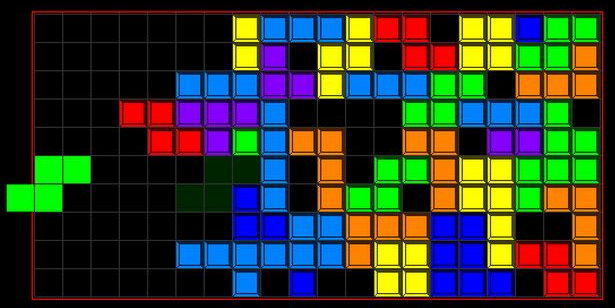
\includegraphics[width=0.65\textwidth]{images/chapter_5_evaluation/tetris_gaps}
    \centering~\caption{A bad attempt at playing Tetris\cite{tetris_gaps}.}
    \label{fig:chapter_5_evaluation-tetris_gaps}
\end{figure}

In conclusion, Table~\ref{table:analysis_results_throttle} and its ensuing analysis suggest that packet throttling is
\textbf{not} working as intended (despite showing some promise) and requires further improvement. Specifically, the
packet throttler needs a better mechanism to ``smooth out'' rough patches such that the aggregate bandwidth is
approximately in line with the configuration. The current algorithm applies a blanket delay to each packet that
passes through it and does not take into account the nuance that the pipeline might be experiencing low traffic. To
use Figure~\ref{fig:chapter_5_evaluation-tetris_gaps} as an analogy, the throttler needs to be better at packet
Tetris and minimise the time gaps between packets as to not overly throttle them.


\section{User Feedback}\label{section:user_feedback}

Six participants were generous enough to spend some of their time to road test Packet Courier and provide feedback.
Four of the participants took part in the user testing phase remotely and expressed their feedback via Microsoft
Forms\cite{microsoft_forms}; the other two provided their feedback in person, which enables notes to be taken as they
were observed interacting with the tool in addition to writing down their comments.

\subsection{Survey Results}\label{subsection:survey_results}

Participants were asked to download a \texttt{.zip} file of the repository before compiling Packet Courier and
completing a selection of tasks. Each of the questions was carefully worded as not to invoke any biases and gave only
the bare minimum context for solving the particular problem. The rationale behind this is that Packet Courier's
\texttt{README.md} should provide users with all the necessary context and troubleshooting information they might
need. Thus, if any of the participants were finding certain tasks unintuitive in a way that the \texttt{README.md}
was failing to address, then this is hugely useful feedback. Conversely, if the survey held their hand during the
entire process, then this defeats the point of collecting feedback on how easy to use and intuitive Packet Courier is
as a tool.

\begin{enumerate}
    \item \textbf{Please describe your occupation, i.e.: Computing Student, Computing Teacher, Network Engineer,
        etc.} \\
    Of the four participants, two where computing students, one was a software engineer and the other a game developer.
    \item \textbf{What platform will you be using to run Packet Courier?} \\
    Two participants were using Windows, one was using MacOS and the other Windows Subsystem for Linux.
    \item \textbf{Packet Courier needs to be compiled using Maven. How would this affect your motivation to use the
    tool? If you are indifferent, please select 5. (Scale from 0 to 10)} \\
    Three participants selected 3; one selected 8. Clearly the choice of project management tool was not particularly
    interesting to the participants.
    \item \textbf{Packet Courier can either be used as a library or executed as a program from the command line. In
    both cases Java 8 (or higher) is required. How would this affect your motivation to use the tool? If you are
    indifferent, please select 5. (Scale from 0 to 10)} \\
    Responses varied quite substantially with participants giving scores of 4, 7, 8 and 10. On the whole, it would
    seem as though participants liked the idea of Packet Courier using Java 8.
    \item \textbf{Packet Courier has no other prerequisites. How would this affect your motivation to use the tool?
    If you are indifferent, please select 5. (Scale from 0 to 10)} \\
    One participant selected 8 while the other three gave a score of 10. It would seem that using software with
    minimal dependencies is a massive upside for users, possibly because of how rare it is for complex tooling such
    as Packet Courier.
    \item \textbf{Please read the Introduction section of the \texttt{README}. Does it concisely convey the purpose
    of the tool and what makes it unique?} \\
    The responses to this question, 7, 8, 8 and 10, would indicate that \texttt{README} introduction is clear and
    informative with a little room for improvement.
    \item \textbf{Please write down any comments or criticisms regarding the Introduction section of the
    \texttt{README}. Is there anything missing? Is anything unclear or ambiguous?} \\
    Participants left a variety of comments in this section, ranging from \emph{``no''} to \emph{``could be a little
    more direct/plain (and therefore shorter)''}. One participant claimed that \emph{``the introduction is clear,
        with enough technical detail that users can understand what is happening but not so much detail that it would
        exclude those with lesser knowledge''}, with another saying that \emph{``uniqueness is not self evident''}
    but that \emph{``a section of the \texttt{README} explaining its benefits over other tools is unnecessary and
    self-indulgent''}. Whilst there is no clear consensus on this particular point (with some of it being down to
    taste), it might be worth investigating ways to trim down the \texttt{README} introduction so that users can get
    stuck straight into the tool. The comments about uniqueness are interesting, perhaps implying that users don't care
    about the unique selling point of a tool by the time they're skimming through the \texttt{README} and that they
    just want
    to get to work actually using it.
    \item \textbf{Please build the project. How complicated did you find this process?} \\
    All participants responded 10 to this prompt, reinforcing the choice to use Maven as the project management tool
    due to its simplicity.
    \item \textbf{Please explain any difficulties you had compiling Packet Courier.} \\
    Only one participant opted to leave a common here and suggested that the \texttt{README} mentions Maven's quiet
    mode to reduce console noise.
    \item \textbf{Please read \texttt{cmd\_example1.courierconfig}. On first glance, does this file read intuitively
    for a network emulation configuration? Suppose you were shown this file for the first time and were only told
    that it was used to configure an emulated network scenario; how well would you understand what the attributes and
    their values were referring to? If you can't find it, then the \texttt{README} should prove helpful.} \\
    Participants responded with scores of 8, 9, 9 and 10, indicating that the \texttt{.courierconfig} file format is
    very user friendly, even to people who are totally new to Packet Courier.
    \item \textbf{If you had to consult the \texttt{README} to get a better understanding of
    \texttt{cmd\_example1 .courierconfig}, then please rate how helpful it was in clarifying any initial confusion.} \\
    Three participants opted to respond to this prompt, all giving a 10 rating.
    \item \textbf{Please write down any comments or criticisms regarding the structure or the contents of
    \texttt{cmd\_example1.courierconfig}. Did the \texttt{README} do a good job at explaining any components that
    weren't self
    evident in their function?} \\
    Two participants suggested that a YAML\cite{yaml} file would make for a cleaner, more human-readable format,
    which seems like a very sensible suggestion. Another participant noted that they had to read up on what
    \emph{``wall-clock''} meant, although the \texttt{README} did help them on that front.
    \item \textbf{Please run a Packet Courier emulation from the command-line using
    \texttt{cmd\_example1.courierconfig} as the configuration. How complicated did you find this process? Note that
    the network code for this configuration uses \texttt{python3}, and is known to work with version 3.8.10.} \\
    Participants gave scores of 7, 8, 10 and 10 for this section. So far it seems as though Packet Courier is being
    received as a very easy to use and highly intuitive tool.
    \item \textbf{Please explain any difficulties you had running a Packet Courier emulation.} \\
    The participants had a lot to say in response to this prompt. \\ \\
    Windows users experienced issues at the level of the operating system whereby double-quotes were stripped from
    Java \texttt{ProcessBuilder} commands\cite{java_ProcessBuilder_double_quote_windows,
        microsoft_docs_main_function}, which in turn prevented the Python scripts from properly parsing the
    arguments. Even after hot-fixing that problem, the Windows kernel seemed to block the packets as a security
    measure. These issues are not bugs or problems with Packet Courier specifically, but operating system quirks that
    must be worked around and troubleshot. The security/firewalling issue can be investigated and discussed in the
    \texttt{README} to help Windows users get the most out of the tool as quickly as possible. \\ \\
    The MacOS user cites that whilst their Packet Courier instance did technically start, it exited nearly
    immediately due to an attempt to bind an ip-address to an existing socket. This is a genuine design oversight
    that has been logged as a known bug. Packet Courier should instead attempt to bind its public and private
    ip-addresses to a socket and retry if they fail instead of presuming that they will succeed. \\ \\
    The WSL user managed to run the simulation in full but expressed how the \texttt{README} was lacking in its
    explanation of how to add loggers to the configuration. They also noted that Packet Courier doesn't create
    missing directories for features such as file logging and crash dumps, which would be a nice quality of life
    improvement.
    \item \textbf{Please briefly examine the simple\_client.py and simple\_server.py scripts that are run as part of
    \texttt{cmd\_example1.courierconfig}. Does the terminal output match what you would expect given the nature of
    the network code and the configuration file? Perhaps consider the order of the messages, as well as if any are
    missing.} \\
    One participant left a long response to this prompt, mentioning how \emph{``I am confused as to why sometimes Bob
    receives a message before Alice seems to have sent it''}. This is a largely unavoidable consequence of multiple
    processes competing for the same console output, however it should probably be mentioned somewhere in the
    \texttt{README}. The participant also suggests \emph{``perhaps more useful log in file form would to have
    separate files for each command node with a timestamp for each line''} since it \emph{``would allow easier side
    to side comparison on a specific message basis''}, which is undoubtedly another excellent feature proposition.
    \item \textbf{What are your general impressions of Packet Courier having used it? (Out of 5 possible stars)} \\
    Participants scored Packet Courier at an average of 4.25 stars.
    \item \textbf{How well do you think your actual experience of Packet Courier matches up to the description given
    in the Introduction of the \texttt{README}?} \\
    Two participants gave Packet Courier a 6/10 on this front, with the other two scored it 8 and 9 respectively.
    This is a surprising outcome in light of previous feedback and it is difficult to pinpoint what is motivating
    this score.
    \item \textbf{If you ever needed to emulate a network scenario, how likely do you think you would be to use
    Packet Courier as your tool of choice?} \\
    Participants gave pleasing ratings on this question: 7, 8, 9 and 10. This paints a picture that even despite the
    technical issues faced by some of the users, they were impressed enough by the presentation of the tool and
    understood its potential enough to overlook issues that could be fairly easily solved.
    \item \textbf{If you'd be hesitant to use Packet Courier again in the future, please explain why.} \\
    One participant left a comment for this prompt, claiming: \\
    \emph{``The lack of a GUI can be daunting for complex structures (e.g. multiple layers of nested topologies) but
    certainly not impossible. As mentioned I haven't seen alternatives but this most certainly does the job it claims
    with great flexibility.''} \\
    Whilst a GUI would certainly address this problem, it would require a significant amount of time and resources to
    develop for a set of fairly niche edge cases. It makes for a compelling suggestion, althougn some research into
    the demand for that kind of functionality might be useful.
    \item \textbf{Please write down any comments or criticisms regarding your experience of Packet Courier as a
    whole.} \\
    The most significant response to this prompt was: \\
    \emph{``As its biggest weakness is in troubleshooting the configuration, and linking with my previous feedback,
        perhaps a GUI tool/form/companion with rigid choices that generates a correct config file could be a useful
        extension.''}
\end{enumerate}

One of the participants went to the extra effort of configuring a couple of emulation scenarios from scratch and
documenting their experience. They said that Packet Courier was \emph{``overall easy to configure''} but had
difficulty debugging mistakes they had made when writing their configurations due to a number of unhelpful error
messages. For example, they had forgotten to place a comma between elements when defining a list of joint-mesh
topologies, to which Packet Courier spat out the following error: \texttt{Configuration error: com.google.protobuf
.InvalidProtocolBufferException: Repeated field elements cannot be null in field: thorpe.luke.network.simulation
.JointMeshTopologyProto.jointTopologies}. Whilst this is a Google Protocol Buffer parser exception rather than an
error message specifically programmed by the Packet Courier APIs, it still plays a role in user experience and thus
should be duly noted. The participant suggests that Packet Courier should use a parser that ignores trailing commas,
since most tooling they had worked with afford the users the luxury of not needing to delimit their lists. This may
be an option, but switching over to a YAML format would negate this problem entirely.

The overall consensus from the survey feedback suggests that users found Packet Courier easy to set up and run due to
a mixture of straightforward tooling, intuitive configuration files and clear documentation. However, there are
issues on Windows and MacOS that prevented some users from running emulations. Despite the fact that Java itself is
largely platform agnostic (and thus Packet Courier did actually \emph{run}), it seems as though the platform-specific
user space APIs do not always manifest themselves uniformly across all operating systems, i.e.: Windows stripping
process commands of double quotes and blocking packets. This is all useful feedback that will inform how Packet
Courier should be developed going forward in Section~\ref{section:future_work}.

\subsection{Observation Results}\label{subsection:observation_results}

Two user observation sessions were conducted to monitor how users \emph{behaved} while interacting with Packet Courier
before interviewing them to get an understanding for their thought processes\cite{user_observation}. The first
interview was done with ``John'' in a more informal manner in attempt to assess what users might expect from the tool
when reading the documentation and example configurations for the first time. The second interview was done more
formally with ``Harry'' to see how a user might debug a network protocol using Packet Courier\footnote{``John'' and
``Harry'' are aliases being used to preserve anonymity.}.

\subsubsection{John}\label{subsubsection:john}

John has a first class degree in computer science and now works as a full time junior software and DevOps engineer.

John was provided with a laptop at the start of the session with an IDE and a WSL terminal open at the root of the
Packet Courier repository. He was also was told that there was a \texttt{README.md} file in the root of the project
directory and was then asked to run an example configuration. John was reasonably comfortable with Java and Maven
since he had done some development with them at university so had Packet Courier built and running fairly quickly. He
was able to identify where the example configurations were based on the \texttt{README}, but said that running them
was \emph{``a bit fiddly''} due to how long the file paths were. The example configurations are buried fairly deep
inside the directory structure of the project and this could definitely be changed to make them more accessible.

John immediately went to run \texttt{cmd\_example1.courierconfig} which suggests that the naming of the example files
is intuitive, i.e.: \texttt{cmd\_example1.courierconfig} is the simplest configuration that can be run from the
command line. He was then prompted to look inside the file he had just run to see if it matched up to what he had
observed on the console. His initial reaction was that \emph{``it looks as though about half of the packets got
dropped, so seems on point''}. John had not even been asked whether he understood the contents of the
\texttt{.courierconfig}; he was instantly able to identify at a glance that about 50\% of the packets travelling from
Alice to Bob were supposed to be dropped. John then reran the simulation to see if it behaved consistently. He
confirmed that whilst the output was non-deterministic, the behaviour of Alice and Bob was still commensurate with
his expectations based on the configuration. He was not put off at all by the fact that sometimes Bob would appear to
receive packets ``before'' Alice, since he understood that the console output was not necessarily running perfectly
in tandem with the underlying client and server processes. In this way, John had built a very strong intuition for
the semantics of Packet Courier quite quickly.

John began to tinker around with the configuration, namely changing the drop probability to 0.9. He was confused to
see that Bob hadn't received any of the packets that Alice had sent. He reran the configuration to find the same
outcome. He then tried running the configuration with a drop probability of 0.3 and found that whilst Bob was
receiving packets from Alice, they were, by eye, less than John would have expected. He then concluded that Packet
Courier must have some kind of packet dropping bug and summarised his experience as follows:
\begin{quote}
    \emph{``I think [Packet Courer] is quite intuitive to use. The configs are quite readable and flexible, in that
    you don't need to fill [a configuration file] with the same amount of complexity each time. It behaves
    consistently and mostly as I would have expected, but there was that weird edge case with the super high and
    super low drops. It could have also benefited from a UI.''}
\end{quote}

Naturally it was disappointing to hear a user conclude that Packet Courier's drop mechanism is buggy given the rigour
of the unit and system testing conducted in Sections~\ref{section:unit_testing} and~\ref{section:system_testing}. The
behaviour that John had uncovered was then promptly investigated. As expected, the root cause of this erroneous
behaviour did not lie within the Packet Courier framework, but was instead a fragility issue in the way Alice and
Bob's connection had been set up in \texttt{cmd\_example1.courierconfig}, the details of which were discussed with
Harry in Section~\ref{subsubsection:harry}. In this way John's feedback had proved invaluable since his curiosity had
led him to discover a hidden edge case in \texttt{cmd\_example1.courierconfig}. Although this was not the result of a
Packet Courier bug, it is still problematic to provide users with examples that could easily convince them that the
framework itself is broken, so this configuration must be made more robust. Otherwise, John seemed to take to using
the tool like a duck to water, with the minor exception of struggling to type out the long path to the example
configurations.

\subsubsection{Harry}\label{subsubsection:harry}

Harry is in his fourth year studying material sciences on an integrated master's programme. Whilst he is technically
competent, he is not a ``seasoned'' software engineer.

Like John, Harry was provided with a computer at the start of the session with an IDE and a WSL terminal open at the
root of the Packet Courier repository. He was also was told that there was a \texttt{README.md} file in the root of
the project directory. Harry was asked to read the introductory sections of the \texttt{README} and provide some
verbal feedback. He noted that \emph{``it is clear what the tool does and [the introduction] provides a nice
overview''} with the caveat that \emph{``packet manipulation seems very core to the tool and could be mentioned
earlier''}. When asked if the introduction left him confused or unclear on any particular point, he responded
\emph{``nothing jumps out as being ambiguous or confusing and the phrase `as though they were running in the real
world' makes me want to read on and figure out what this entails''}. As such, it seemed as though Harry was more
intrigued by the introductory sections of the \texttt{README} than anything else.

Harry had never used Maven before and asked if \emph{``Maven was to Java what pip\cite{pip} is to Python''}. He also
added that it wasn't immediately obvious to him what the \texttt{-DskipTests} option recommended in the
\texttt{README} had to do with compiling the project. Comments like this are highlight that most developers take this
kind of information for granted and perhaps the \texttt{README} could be subtly tweaked to be friendlier to those who
are newer to the paradigm. Harry also mentioned that the initial build process spammed the console with lots of
\emph{``very intimidating''} text. This links back to some of the survey feedback from
Section~\ref{subsection:survey_results} that suggested using Maven's quiet mode when compiling.

When Harry was asked to run an example configuration, he had a look through the \texttt{README} and initially
attempted to use the Google Protocol Buffer grammar, i.e.:
\texttt{src/main/proto/packet\_courier\_simulation\_configuration.proto} in place of a configuration file. It seems as
though the \texttt{README} makes it too easy for all of the various paths to be confused for one another and the
brevity of this section results in potential ambiguity, particularly for first time users. Just as with John, Harry
expressed how he felt as though the path to example configurations was unreasonably long. Indeed, he did need several
attempts to get the command right as a consequence of this, but each time Packet Courier gave him an error message to
let him know that the path wasn't correct. This then led him to conclude that \emph{``even if I hadn't realised I was
trying to run the grammar rather than a config file, Packet Courier would have told me it was the wrong kind of file
anyway, so it's not a big problem''}.

Just like John had done, Harry went straight to \texttt{cmd\_example1.courierconfig} as soon as he had found where
the example configurations were stored. He immediately observed that Bob had received Alice's packets out of order
and on some occasions, had received these packets before Alice had sent them. He wasn't concerned by the latter issue
though, since he chalked it up to \emph{``display issues; it's not really indicative of what's going on
underneath''}. Before inspecting the configuration file itself, Harry reran the emulation to see if it was
deterministic. He realised that whilst the exact output wasn't the same as before, the underlying behaviour seemed to
be approximately the same. This time, however, he saw that some packets were missing and decided to look at
\texttt{cmd\_example1.courierconfig} for an explanation.

Harry instantly identified \texttt{cmd\_example1.courierconfig} as having a \emph{``JSON structure''} with an
\emph{``8/10 for clarity; even scanning through the file, terms like `drop probability' leap out of the screen''}. To
supplement his understanding, Harry then compared what he was reading to the \texttt{README} and had a brief look at
\texttt{simple\_server.py} and \texttt{simple\_client.py}. He was not prompted to do this. He then claimed to
\emph{``now fully understand what came out of the terminal''}.

Just as with John, Harry then began to fiddle around with the parameters of \texttt{cmd\_example1.courierconfig},
setting packet drop probability to 0.7. Harry noticed that Bob was receiving none of Alice's packets and ran the
emulation a second time to verify that this wasn't \emph{``just an unlucky run''}. His instinct was to then consult
the \texttt{README} in case there was any supplementary information which could explain why this might be happening.
He conjected that he might have misunderstood what the \texttt{dropProbability} meant, but having realised that it was
effectively a Bernoulli parameter, he decided to experiment further with the probabilities. He found that a drop
probability of 0.6 would result in Bob receiving about 100 packets, but 0.65 would see Bob receive none. Harry
suggested that there was some kind of \emph{``minimum number of packets''} that Bob needed to receive in order to
display his output.

In light of this new hypothesis, Harry chose to remove all network conditions to ensure that every packet being sent
by Alice \emph{should} get through to Bob. This test run showed Bob receiving about 200 packets instead of the full
250. Harry then concluded that the packets appeared to be coming in groups of 100, but admitted that his lack
of technical knowledge preventing him from understanding exactly why this was happening.

It turns out that Bob would receive packets in groups of 101 specifically, which was discovered by changing the
number of packets Alice was sending and figuring out the exact threshold for when Bob started to receive them. The
packets in this configuration were 32 bytes long. This combined with UDP's header size of 8 bytes makes each full
packet 40 bytes long. Notice that $101 \times 40B = 4040B \approx 4KiB$ which just so happens to be the default page
size for Linux\cite{default_page_size}. The \texttt{getconf PAGESIZE} command\cite{linux_page_size} revealed that
this WSL instance did have a page size of 4096 bytes, which would explain why Bob would only receive his packets once
approximately that specific quantity had accrued, namely since most transfers between buffers are page-wise
operations at the level of the kernel\cite{paging}.

Whilst Harry wasn't able to come up with insights that were as precise as the explanation provided above, he was able
to use Packet Courier to identify this behaviour at a high-level, i.e.: Bob was only receiving Alice's packets in
bursts of around 100, despite not being from a software engineering discipline. He concluded the session by stating:
\begin{quote}
    \emph{``This has actually changed my mind about this sort of thing. Usually if I were investigating how some
    hardware behaved, I'd probably want to run some tests that gave me a load of aggregated statistics at the end of
    it. In this case I'd guess it'd be stuff like delay or drop rate. However seeing the packets printed individually
    like this has allowed me to spot patterns in how they arrive, especially since you can just tweak the network
    conditions really easily. Although, the structure of the config file itself could be friendlier.''}
\end{quote}


\section{Analysis of Objectives}\label{section:analysis_of_objectives}

In light of all the quantitative evidence gathered during unit and system testing, and the qualitative evidence
presented using user testing iterations, Packet Courier can now be judged on how well it has completed the objectives
laid out in Section~\ref{section:objectives}.

\subsection{Network Topology Design Interface}\label{subsection:network_topology_design_interface}

\textbf{Objective 1:} \emph{An interface to design an arbitrary network topology.} \\

Packet Courier has demonstrably completed this objective. Users can (and have been shown to during user trials)
design their own custom network topologies as part of Packet Courier, which they can then later layer network
conditions on top of. This can either be achieved using the simulation APIs discussed in
Section~\ref{subsection:simulation_api} or using the Google Protocol Buffer integration discussed in
Section~\ref{subsection:protocol_buffer_integration}.

Whilst this functionality does objectively exist within the Packet Courier framework, user feedback suggests that a
GUI would improve quality of life as it would enable users to visualise their topology more vividly. Not every
developer would want to use a GUI, but there is clearly a demand for a feature like this and adding a more visual
interface for users would certainly broaden the appeal of the tool.

Another common theme among user feedback is that the structure of \texttt{.courierconfig} files could be cleaner,
perhaps adopting a YAML\cite{yaml} format that disposes with braces, for example. The error messages that users
receive when their topology is incorrectly configured could also be improved.

In conclusion, Packet Courier \textbf{does} achieve this objective, although there is still scope to improve the
quality of its delivery to users.

\subsection{Network Conditions Configuration Suite}\label{subsection:network_conditions_configuration_suite }

\textbf{Objective 2:} \emph{A configuration suite to define how packets are manipulated during message-passing.} \\

Packet Courier has demonstrably completed this objective. Users can (and have been shown to during user trials)
specify their own custom network conditions. In fact, user feedback suggests that this is one of Packet Courier's
strengths, in that the parameters encoding for the details of a network condition are very clear and intuitive.
Packet Courier provides parity with the existing tool \texttt{tc-netem}\cite{tc_netem_wiki, tc_netem_8_man} as per
Section~\ref{subsection:network_condition_semantics}, but has also gone further to incorperate event-based semantics,
as detailed in Sections~\ref{subsection:event_based_semantics} and~\ref{subsubsection:simulated_event_pipeline}.

In conclusion, Packet Courier \textbf{does} achieve this objective.

\subsection{Simulation of a Distributed Algorithm}\label{subsection:simulation_of_a_distributed_algorithm}

\textbf{Objective 3:} \emph{A mechanism to run a distributed algorithm across a virtual network topology which
reflects the properties described by the user as per objectives 1) and 2).} \\

Packet Courier has demonstrably completed this objective. Users can (and have been shown to during user trials)
specify their own simulation and emulation scenarios as per the topology and network condition interfaces and APIs
mandated by objectives 1) and 2).

Packet Courier offers users the ability to run their configurations as simulations in the form of Java code or
emulations using UDP sockets to communicate with arbitrary processes.

The system tests show that five of Packet Courier's six base network manipulation tools operate to a high level of
engineering precision. Despite the fact that bandwidth throttling does go some way to fulfilling the obligations
outlined in Section~\ref{subsection:network_condition_semantics}, the data in
Table~\ref{table:analysis_results_throttle} and its associated analysis in
Section~\ref{subsubsection:throttle_analysis} show that it is imprecise and demands further refinement.

In conclusion, Packet Courier \textbf{does} achieve this objective, although one of the six core networking features
needs further iterations before it could be considered ``engineering grade'' by any reasonable metric.

\subsection{Platform Agnosticism}\label{subsection:platform_agnosticism}

\textbf{Objective 4.a:} \emph{Basic usage of the tool should not depend on the operating system or hardware being
used .} \\

While in principle Packet Courier does \emph{run} on Windows, MacOS and Linux, there are blocking issues on Windows
and MacOS that are not accounted for in the source code, nor do they have appropriate troubleshooting prompts in the
\texttt{README}. These are problems that will certainly be ironed before the second iteration of user feedback, but
as Packet Courier stands at the time of writing this report, these bugs exist and are listed as known issues on the
project Kanban board.

In conclusion, Packet Courier \textbf{does not} achieve this objective. \\ \\

\textbf{Objective 4.b:} \emph{Users should not be pigeonholed into working with a particular programming language in
order to simulate their solution.} \\

Packet Courier has demonstrably completed this objective. Users can (and have been shown to during user trials) use
languages such as Python to write their net-code for Packet Courier emulations. Indeed, the very examples provided in
GitHub repository use \texttt{python3}. The UDP based design pattern outlined in
Section~\ref{subsection:emulation_semantics} enables developers to use any \emph{arbitrary binary} that they might
wish to, let alone their preferred programming language.

In conclusion, Packet Courier \textbf{does} achieve this objective.

\subsection{Plug-and-playability}\label{subsection:plug_and_playability}

\textbf{Objective 5.a:} \emph{Users should need minimal domain-specific knowledge in order to use the full set of
features on offer.} \\

Packet Courier has demonstrably completed this objective. Users can (and have been shown to during user trials)
design and run their own custom Packet Courier emulations by simply referring to the \texttt{README} as a glorified
glossary of terms.

A common piece of user feedback is that virtually all of Packet Courier's external elements were fairly
self-explanatory, whereby no complex knowledge or extensive study of documentation is required to get an emulation up
and running. Even Harry (the user testing participant observed and interviewed as part of
Section~\ref{subsubsection:harry}) was able to enjoy Packet Courier's offerings as material science student with
only a baseline technical competence.

On balance, users did specify areas where documentation could be improved, namely with regards to troubleshooting.

In conclusion, Packet Courier \textbf{does} achieve this objective, although the \texttt{README} could still do with
some refinement. \\ \\

\textbf{Objective 5.b:} \emph{The prospective tool should be able to mimic a real network in a way that minimises
bespoke set-up, i.e.: if a user normally tests their distributed algorithm using real computers connected over a
physical network, then transitioning to using the prospective tool should be more or less seamless.}

Packet Courier has demonstrably completed this objective. Users can (and have been shown to during user trials) use
Packet Courier as a silent process that works in the background to emulate a network that routes UDP packets. This is
discussed in detail as part of Section~\ref{section:standalone_emulator}.

In conclusion, Packet Courier \textbf{does} achieve this objective.